\documentclass[11pt, oneside]{article}   	% use "amsart" instead of "article" for AMSLaTeX format
\usepackage{geometry}                		% See geometry.pdf to learn the layout options. There are lots.
\geometry{letterpaper}                   		% ... or a4paper or a5paper or ... 
%\geometry{landscape}                		% Activate for rotated page geometry
\usepackage[parfill]{parskip}    		% Activate to begin paragraphs with an empty line rather than an indent
\usepackage{graphicx}				% Use pdf, png, jpg, or eps§ with pdflatex; use eps in DVI mode
\usepackage{caption}
\usepackage{subcaption}
\graphicspath{ {Users/hld523/Reports/my-plasma-report/Figures/} }								% TeX will automatically convert eps --> pdf in pdflatex		

\usepackage{amssymb}
\usepackage{amsmath}

%SetFonts

%SetFonts


\title{Plasmaaaaa}
\author{The Author}
%\date{}							% Activate to display a given date or no date
\begin{document}
\maketitle
\section{Introduction}

\subsection{Reactive Oxygen and Nitrogen Species in Biology}

Reactive oxygen and nitrogen species are highly reactive molecules, which include free radicals and other non-radical species. 
Free radicals, such as hydroxyl and superoxide radicals, are atoms or molecules with a single, unpaired electron in their outer shell \cite{PhamHuy2008}. 
This free electron results in an extremely high propensity to react with molecules nearby. 
In biological settings, these species are capable of attacking proteins, lipids and DNA \cite{PhamHuy2008} which can lead to their deleterious effects such as mutations.
Other highly reactive molecules such as ozone and hydrogen peroxide are not free radicals in that they do not have an unpaired electron in their outer shell, however, they are still strongly reactive and are capable of reacting to produce free radicals \cite{PhamHuy2008}.

In the past, it was thought that these RONS were solely damaging molecules present in the body that led to ageing and age-related diseases.
These thoughts were termed the free radical theory of ageing \cite{Harman1955}. 
However, since then, it has been shown that, whilst RONS do have a large role in many pathologies, such as diabetes, cardiovascular disease and neurodegenerative disorders, amongst many others \cite{Valko2007}, they are also believed to be important molecules involved in normal physiological functioning.
Of particular interest is the role of free radicals in bacterial killing during an immune response.
Certain immune cells, known as phagocytes, whose job it is to engulf and kill invading pathogens, produce free radicals and other reactive species, such as superoxide, hydrogen peroxide and hydroxyl radical, to kill the engulfed pathogen in a process known as the respiratory burst \cite{Janeway2011}
The importance of this process is shown by patients with chronic granulomatous disease who lack the enzyme required for superoxide production. This means their immune cells cannot produce superoxide in the respiratory burst and predisposes the individual to multiple, persistent infections \cite{Janeway2011, Babior2004}.


This ability to kill bacteria, has led to the idea that these reactive species may provide a potential alternative to conventional bactericidal therapies such as antibiotics, the resistance to which is proving to be a huge challenge in the world today. 
By understanding the role of RONS in the normal functioning immune system, it my provide details of how we could manipulate these species for use in biomedical applications such as bacterial killing in chronic or infected wounds.
However, in order to do this, there would need to be a mechanism for producing and administering the RONS in suitable concentrations.
This is an issue due to the short lived, highly reactive natures of the species.
Recently, there has been much research into the development of low temperature atmospheric pressure plasma jets, which are plasma sources operated at temperatures that are low enough to not be damaging to biological samples, such as the skin, and are potent producers of RONS. 
Low temperature plasmas and their production of RONS will be the focus of the rest of this project.


%RADICALS KILL STUFF, THEREFORE, USE PLASMA!!

\subsection{What is plasma?}
Plasma is ionised gas.
It follows the sequence (with increasing energy) of solid $\rightarrow$ liquid $\rightarrow$ gas $\rightarrow$ 
as a solid becomes liquid and a liquid becomes gas, if energy is increased further, a gas ionises and becomes plasma and therefore, plasma is classed as the fourth state of matter \cite{Fridman2013PlasmaMedicine}. 
The process of ionisation of gases results in free electrons within the plasma region, which gives the plasma it's properties.
The degree of ionisation of a plasma refers to the proportion of gas molecules that are ionised.
This depends largely on the energy of the system. 
The higher the energy, the greater the degree of ionisation and therefore the higher the density of free electrons (electron density).
Plasmas are said to be quasi-neutral, meaning that whilst they contain many charged particles, overall, there is no charge to the system.

\subsection{Low Temperature Atmospheric Pressure Plasmas} \ref{section:LowTempPlasmas}

Plasmas can can range from being almost fully ionised, to very weakly ionised.
Highly ionised, very hot plasmas, such as those forming lightening in nature, exist at very high overall temperatures. 
This is due to a state of thermodynamic equilibrium being reached. 
For this to occur, free electrons are accelerated across a potential difference and gain energy which they then impart to other ions and neutral through collisions.
Although energy transfer between very small electrons and much bigger neutrals and ions is poor, if there is sufficient energy in the system, then all the particles within the plasma will end up 'hot', $T_e \approx T_i \approx T_g$ (where $T_e$ is electron temperature, $T_i$ is ion temperature and $T_g$ is gas temperature).

However, at the other end of the scale are low temperature plasmas. 
These plasmas are only weakly ionised and therefore have low degrees of ionisation and low electron densities.
For these plasmas, thermodynamic equilibrium is never reached due to the poor energy transfer between electrons and bigger ions and neutrals. 
This results in a state where $T_e >> T_i \approx T_g$ and therefore, overall, the temperature of the plasma remains cool at approximately room temperature.
It is this ability to produce plasmas at low temperatures that makes them so exciting in the field of biomedicine and only these types of plasmas will be considered from now on in this report.

Electrons in plasma have a range of energies which forms an electron energy distribution function (EEDF) as shown in ADD FIGURE HERE.
The three main processes that electrons mediate are:
\begin{itemize}
\item Dissociation - electron impact causes splitting of molecules. This is the mechanism by which, for example, molecular gases become atomic and how free radicals can be produced
\item Electronic excitation - electron impact can excite an atom/molecule by causing one of it's electrons to be promoted to a higher energy orbital if the impacting electron's energy matches the difference in energy between orbitals. Following this, the atom/molecule can relax back to a lower energy level, and in doing so, emits a photon with energy equivalent to the difference between energy levels. This is how the visible light from plasma is emitted
\item Ionisation - If the electron energy is sufficient, on collision with another atom or molecule it can cause an electron to be knocked off the particle and result in it's ionisation and a free electron being released. This is the mechanism by free electrons are always being produced in order to sustain the plasma and counteract the loss of electrons due to recombination.
\end{itemize}

Electrons in low temperature plasmas have typical mean energies in the range of 0.5 - 5 electron volts (eV), much greater than energies of larger neutrals and ions (0.025 - 0.05 eV), but much less than the energies required for dissociation, electronic excitation and ionisation \cite{Christophorou2012}.
However, a small fraction of the electrons are able to attain energies sufficient to carry out these processes and therefore sustain a plasma.

\subsection{RONS in plasmas}

Dissociation occurring in the plasma results in large quantities of free radicals and other reactive species being produced and herein lies the potential for using low temperature plasmas for bacterial inactivation \cite{Graves2012}.
These plasmas operate at a temperature that is not harmful to biological samples and can therefore be applied directly to skin, whilst retaining the ability to produce a plentiful supply of RONS. 
The types of RONS produced by the plasma depend on the feed gas and the power supplied to the plasma.
For example, a helium feed gas with admixtures of oxygen will yield reactive oxygen species such as ozone, superoxide and singlet delta oxygen, whereas nitrogen admixtures would yield reactive nitrogen species. 
Being able to tune plasmas is a key step for moving forward with this field of research 

Plasmas need tuning for use on people... Need to know how to produce specific species in specific quantities...


\subsection{Biomedical Applications of Low Temperature Plasmas}

\begin{itemize}

\item One reason for the booming research interest into low temperature plasmas is the potential for biomedical applications of these plasmas.
\item Plasmas have been used in the field of biomedicine for sterilisation, cauterisation etc in the past. However, these plasmas operate at temperatures which exclude them from being used directly on biological tissues, such as the skin.
\item Low temperature plasmas mean that this is no longer an issue as they operate at non-harmful temperatures meaning that they can be used directly in contact with biological samples. 
For example KinPen and PlasmaDerm \cite{BrehmerHD2015}....

\item The potential biomedical applications come from the fact that these plasmas are a source of UV radiation, electrical fields and, of particular interest to this project, they are a potent source of reactive oxygen and nitrogen species. All of these things have potential to influence biomolecules such as DNA which can in turn play a role in killing of bacteria, for example to promote wound healing, or killing of cancer cells, to provide an alternative to conventional therapies. 
The multimodal nature of plasma treatment could mean that resistance to treatment by it may not occur. 
This would be beneficial in this era of increasing antibiotic resistance.

\end{itemize}

\subsection{The Hydroxyl Radical ($\cdot$OH)}

$\cdot$OH is the most reactive oxygen radical known and reacts very rapidly with nearby molecules \cite{Halliwell2007}. 
Action...

\subsection{Biologically relevant concentrations of hydroxyl radical}

When considering the tuning of plasma jets for biomedical purposes, it is necessary to consider the biologically relevant levels of RONS.
Data for this comes from current literature where quantification of $\cdot$OH radicals comes from different methods such as absorption spectroscopy, electron paramagnetic resonance spectroscopy (EPR) and predictive modelling.

??$\cdot$OH CONCENTRATIONS IN PHAGOCYTES DURING IMMUNE RESPONSE??

Next, by using EPR and a 5,5'-dimethyl-1-pyrroline-N-oxide (DMPO) spin trap (to bind to the short lived $\cdot$OH radical to extend it?s lifetime while remaining a radical), \cite{Zweier1988} investigated the concentrations of $\cdot$OH radicals causing cell death in foetal bovine aortic endothelial cells which had been exposed to anaerobic conditions for a specified period of time before being reoxygenated. EPR was then performed to determine the concentration of $\cdot$OH. Simultaneously, cell samples were taken to test their live/dead status using trypan blue (staining with trypan blue indicates cells are dead). It was found that 10 minutes after reoxygenation, 90\% of cells were staining with trypan blue and this correlated to a $\cdot$OH concentration of 0.3?M. 
%(My molarity is 3 x 10\textsuperscript{-10}).

On the other hand, another group \cite{Attri2015} has investigated, using UV absorption spectroscopy, the density of .OH radicals required to kill lung cancer cell lines using a low temperature plasma jet. For this, cells of the H460 lung cancer cell line were plated on to petri dishes with differing depths of phosphate buffered saline (PBS). The plasma jet was then positioned above the sample and the $\cdot$OH radical density produced within the PBS was measured by UV absorption spectroscopy. For this, a quartz filter was used just below the surface of the PBS which blocked any plasma derived species from entering the solution and only UV could pass through the filter and cause dissociation of water molecules into $\cdot$OH radicals. Following plasma treatment, the cells were then stained with propidium iodide to determine whether they were live or dead. When cells were 2mm below the surface of PBS, approximately 70\% of the original cells stained positive for PI, showing that they were dead.  At this depth, the density of $\cdot$OH radicals was found to be 1.9 x 10\textsuperscript{16} cm-3.  
%(My densities are x 10\textsuperscript{20} m\textsuperscript{-3})

In 2004, Cho et al \cite{Cho2004} investigated the concentration of $\cdot$OH required for a 2-log inactivation of E. Coli during photocatalysis using $TiO_2$ for water treatment. After concluding that $\cdot$OH was the main biocidal component for this kind of water treatment, the levels of $\cdot$OH required for bacterial inactivation could be determined.
$\cdot$OH concentrations were predicted using the delayed Chick-Watson model which relates the decrease in the E. Coli population to the concentration of $\cdot$OH radicals and contact time of the radicals to the bacteria \cite{Cho2003}. Using this model, the concentration of $\cdot$OH $\times$ the contact time of $\cdot$OH with water required to produce a 2-log E. Coli inactivation was predicted to be 0.8 x 10\textsuperscript{5} mg min/l.  Therefore, for a treatment time of 1 minute, a concentration of 0.8 * 10\textsuperscript{5} mg/l of $\cdot$OH is required. 




\subsection{Measuring Hydroxyl Radicals in Plasma}

Different ways of looking at $\cdot$OH concentration in plasmas...

\subsection{Project Hypotheses and Aims}

The ability to fine tune plasmas so that they produce a well characterised range of RONS is key for their development for biomedical applications.
In order to do this, RONS must be characterised individually and the effects of changing plasma parameters on their production, lifetime and decay must be understood in order to be able to manipulate the plasmas to produce the required mixture of RONS.

The aim of this project is to look at the concentrations of $\cdot$OH produced in a low temperature radio frequency plasma and investigate how different plasma parameters such as power and water content affect the production of $\cdot$OH, as well as considering how the position within the plasma channel affects the concentration of $\cdot$OH.
It is hypothesised that increasing the power and water content of the plasmas will be able to increase the densities of $\cdot$OH produced, this would be due to the increased energy supplied by increasing the power and the increase in availability of water to be dissociated.

Further to this, the concentrations seen in these experiments may then be compared to the current literature to start to understand whether the densities produced by this particular plasma may be biologically relevant.


\section{Materials and Methods}

\subsection{Plasma Source}
The plasma source (described previously \cite{Niemi2013}) used consists of two plane-parallel electrodes which are 30mm long and 11mm wide. 
The gap between the electrodes is 1 mm and the gaps at either side are covered by ultraviolet (UV) transparent windows, thereby forming a channel for plasma formation with dimensions of 1 x 11 x 30 mm.
One electrode is driven by a 13.56 MHz radio frequency (RF) generator via an impedence matching box, whilst the other electrode is grounded. 
The helium feed gas used in the plasma can consist of a mixture of dry and humid helium. Humidification of the gas can be achieved by diverting some of the helium through a bubbler (a closed water-containing chamber) in order to pick up water vapour before rejoining the original flow and carrying on to the plasma source.
The dry and humid helium flows were controlled by two separate mass flow controllers.
The gas inlet to the source is at the bottom of the plasma channel and the gas travels through the 30 mm long channel to the gas outlet and is removed by an extractor.




\begin{figure}
    \centering
    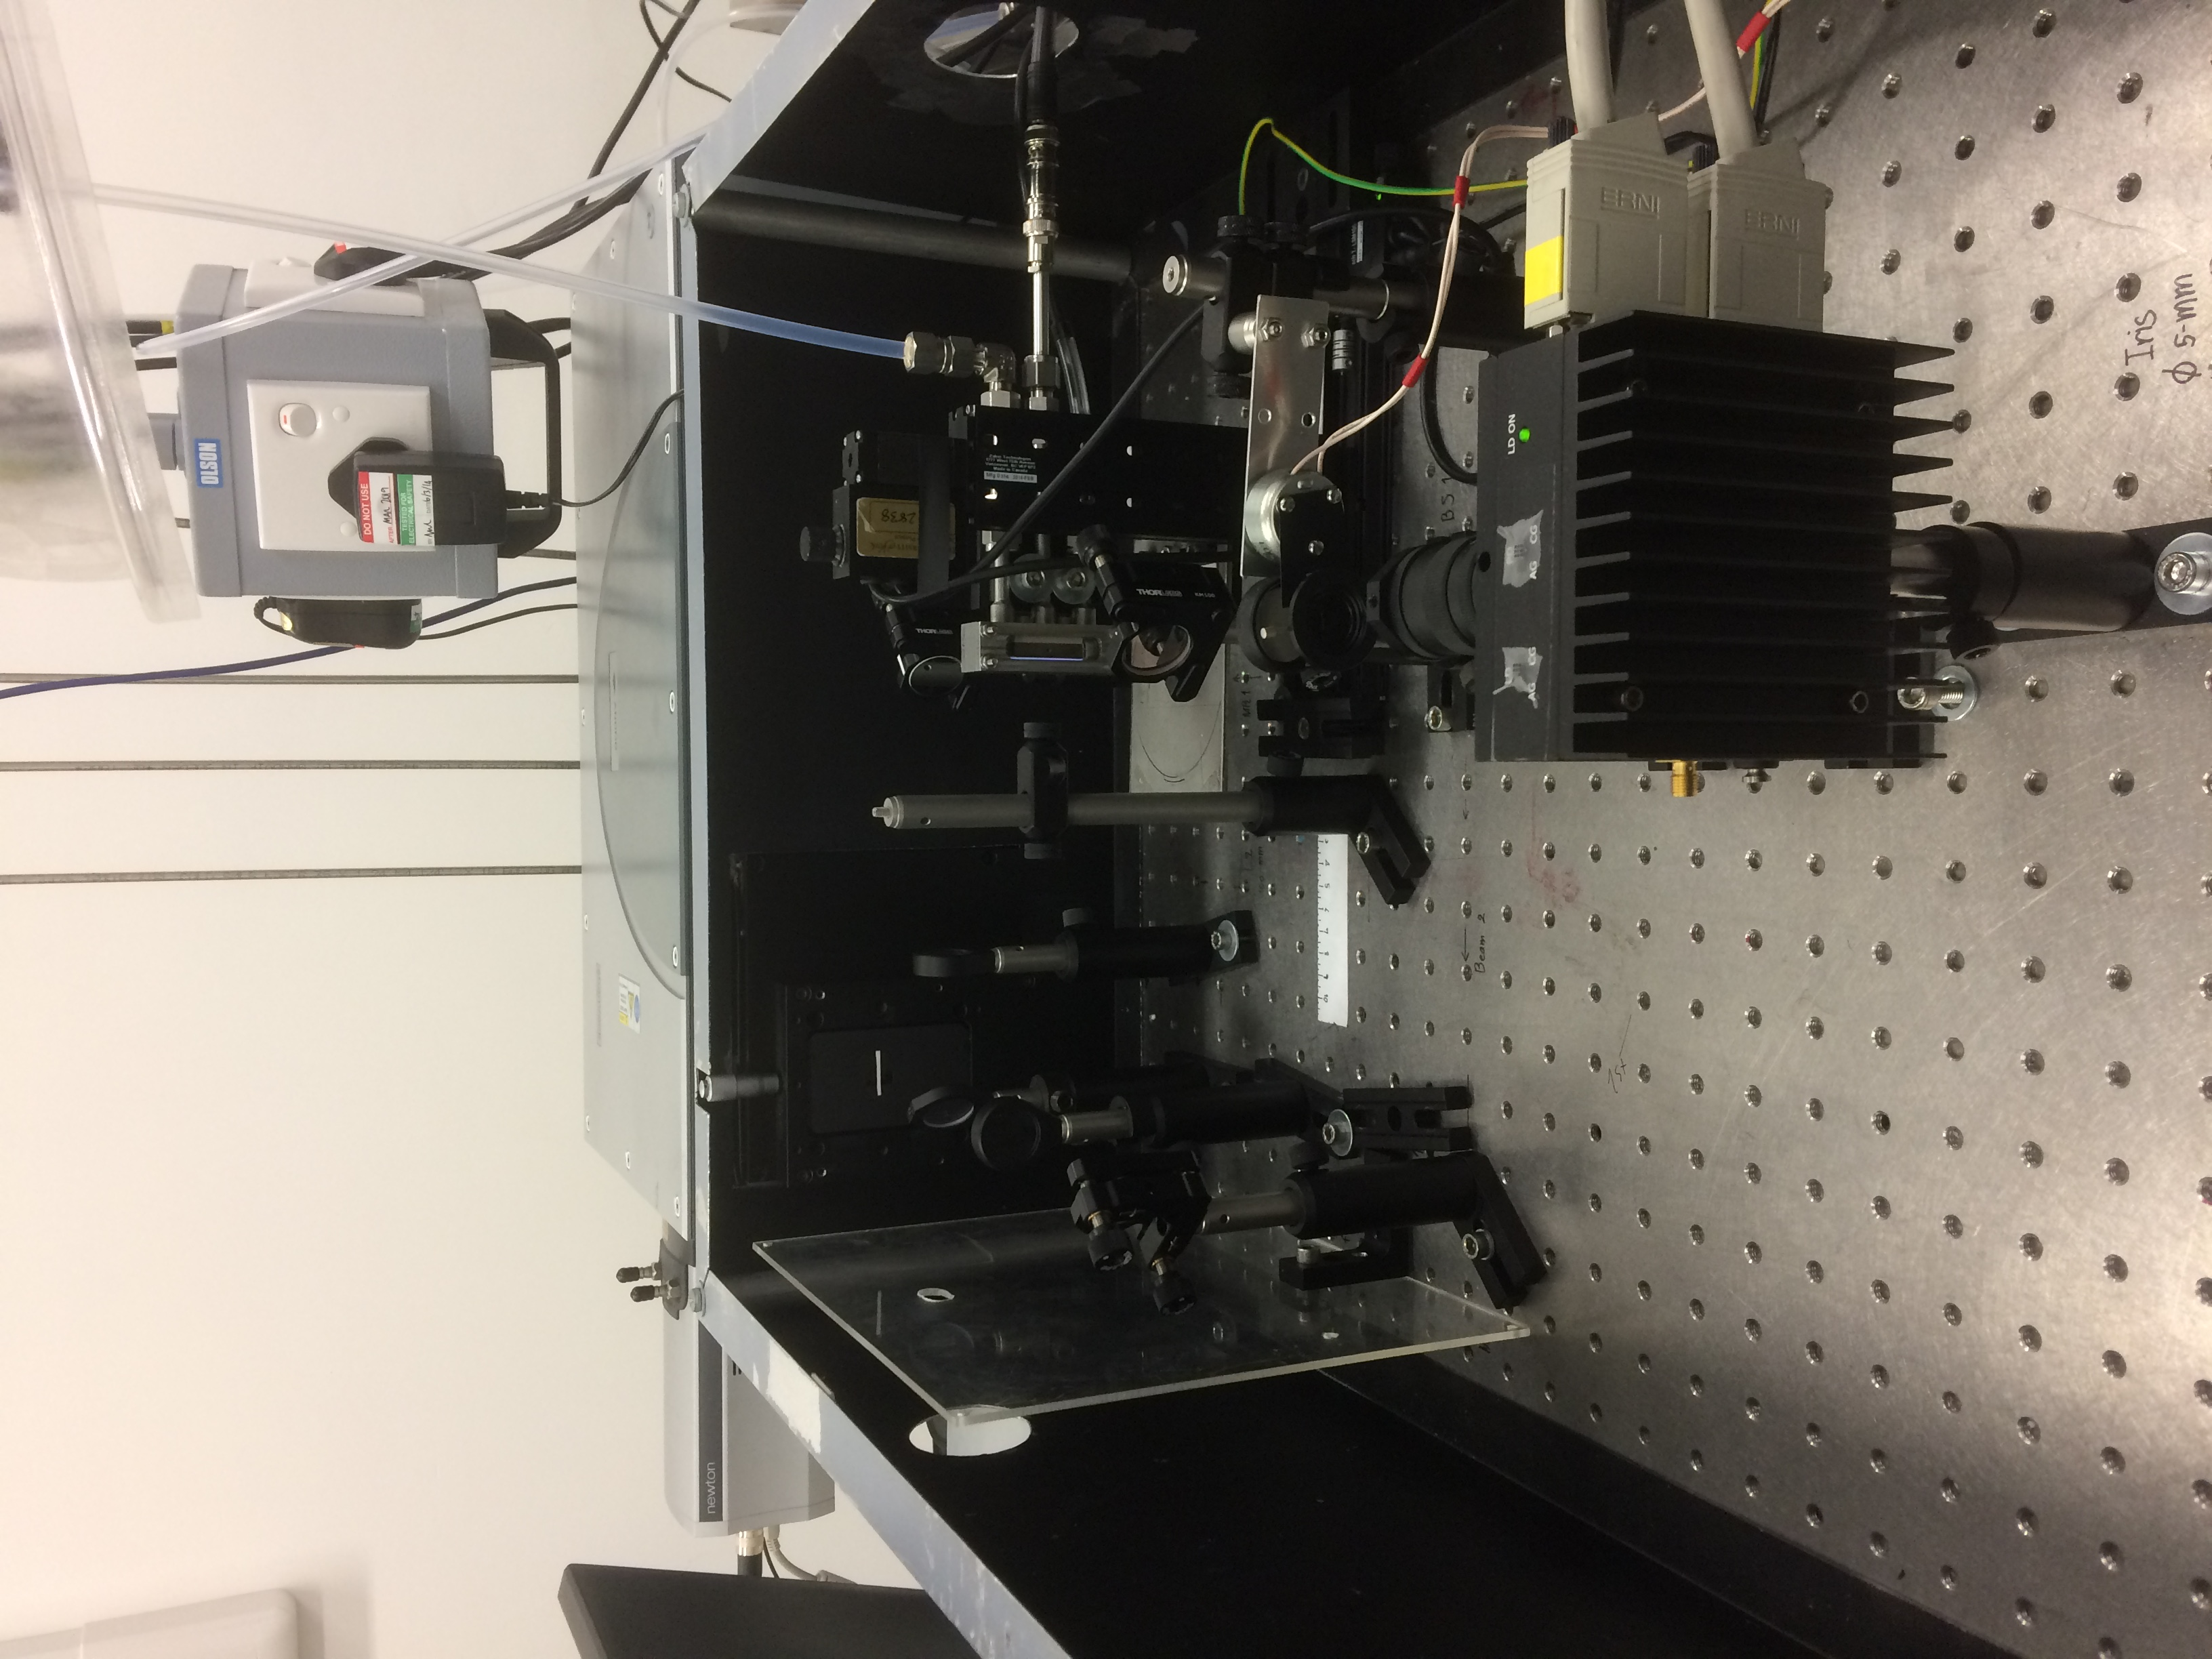
\includegraphics[width=\textwidth]{Figures/PlasmaSetup.JPG}
    \caption{Plasma Setup...This will be a proper diagram...}
    \label{fig:my_label}
\end{figure}


\subsection{Power Measurements}

Whilst the RF generator gives an indication of the power being supplied to the plasma source, it is not very accurate and is unable to account for power losses in cables and other equipment.
To counteract this, the actual power delivered to the plasma can be accurately measured using voltage and current probes connected between the matching box and the plasma source. 
Using these probes, the power supplied to the plasma can be accurately assessed using the equation:

\begin{equation}
P = I \times V \times cos\theta
\end{equation}

where $P$ is power, $I$ is current, $V$ is voltage and $\theta$ is the phase difference between the voltage and current (calculated by connecting the setup to a capacitor with a known phase difference, to which the voltage and current measurements can be compared).
Measurements are taken firstly with the plasma on, then with the plasma off to calculate power lost in the equipment, then finally with the capacitor connected.
The actual power is then determined by using the equation above then subtracting the background losses (obtained during the plasma off measurements), from the measurements with the plasma on.

Using this, the actual power delivered to the plasma was calibrated to the output stated on the output dial (see figure \ref{fig:OutputDial}) of the RF generator. 
This was done by changing the output from 50 - 200 in steps of 10 on the RF generator output dial.
For this, the plasma was operated with a gas flow of 5 slm helium containing 5400ppm water.
This calibration is shown in figure \ref{fig:SolaylPower}.
The relationship between the output and actual power showed a linear relationship and by fitting a line to the measured data, the actual power delivered to the plasma for each output value can be predicted using the line with equation y = 0.1127x - 0.0437 fitted to the data.
All powers stated in this report are real powers calculated from this calibration.

\begin{figure}
    \centering
    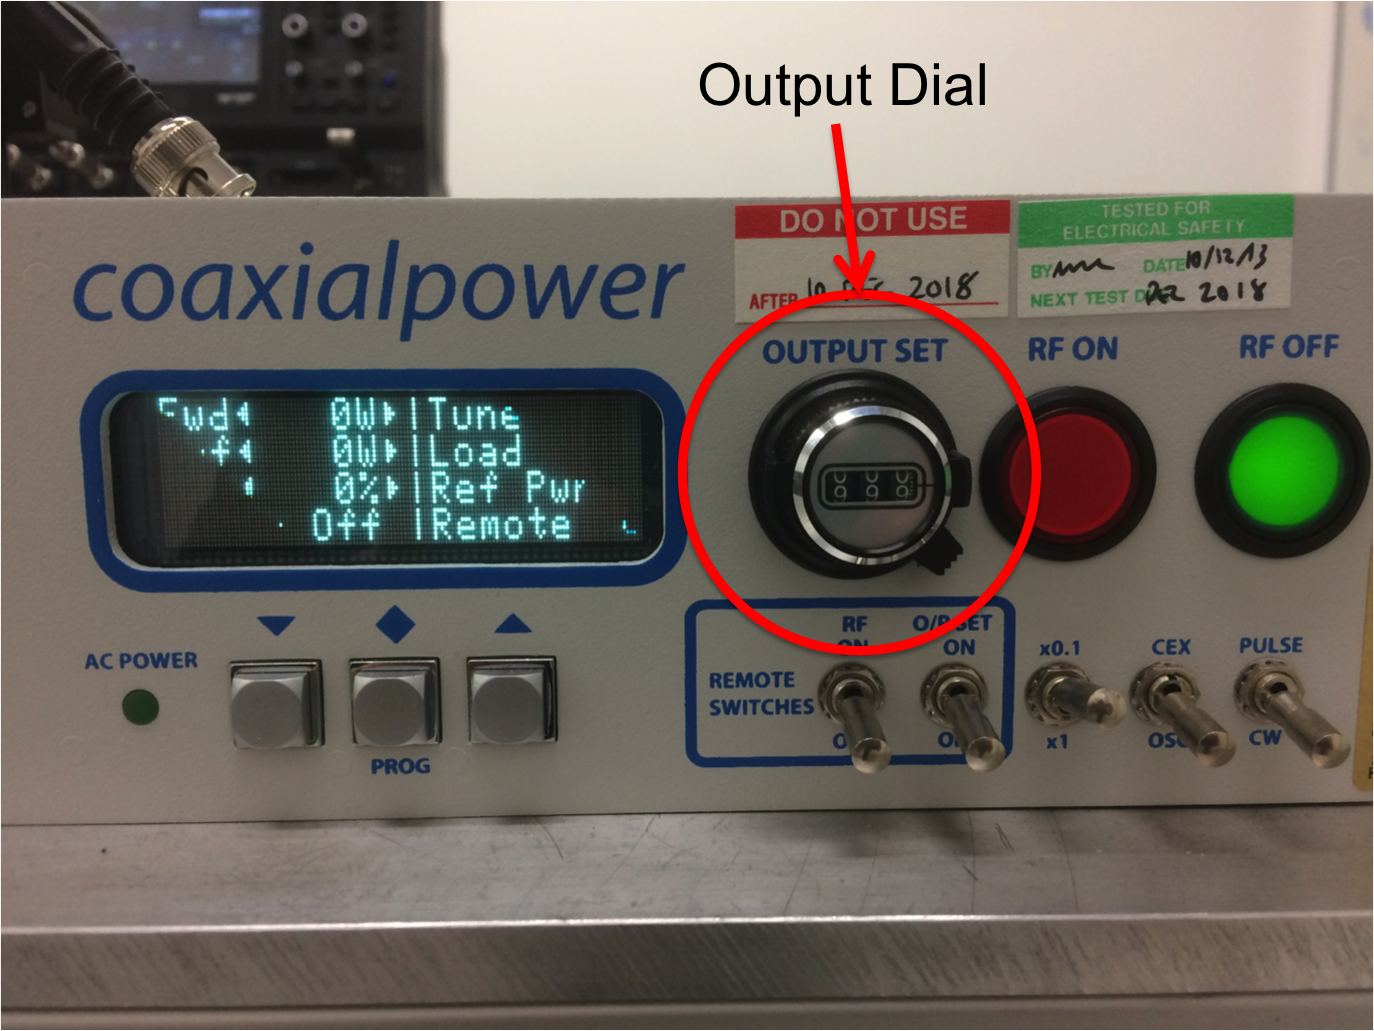
\includegraphics[width=0.4\textwidth]{Figures/OutputDial.png}
    \caption{Picture showing the Output dial on the RF generator used for calibrating output from the RF generator to the actual power supplying the plasma}
    \label{fig:OutputDial}
\end{figure}

\begin{figure}
    \centering
    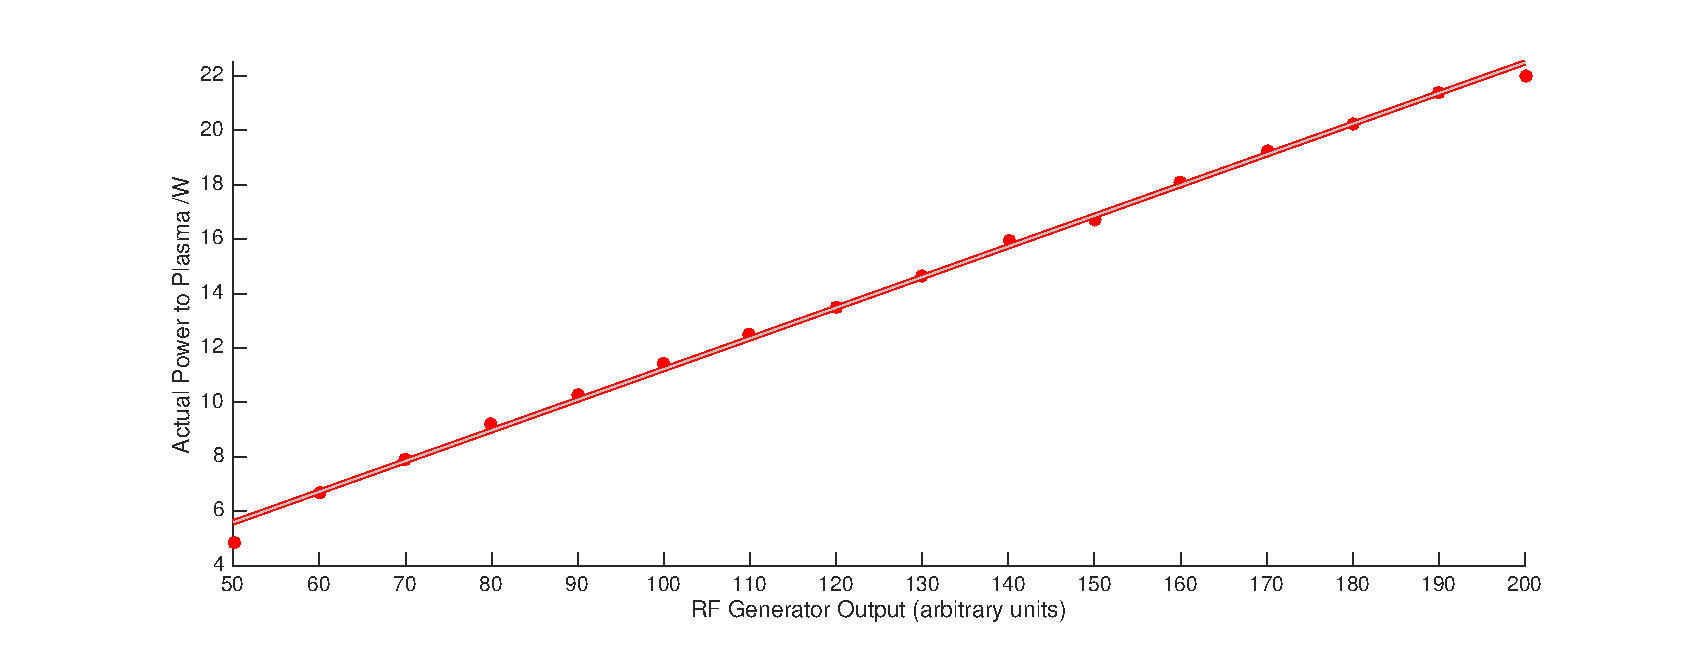
\includegraphics[width=\textwidth]{Figures/ActualPower.eps}
    \caption{There is a linear relationship between the output on the RF generator and the actual power supplied to the plasma. The x axis shows the value for the output on the RF generator (see figure \ref{fig:OutputDial} in arbitrary units and the y axis shows the corresponding power supplied to the plasma, corrected for losses in equiment. The line of best fit shown has the equation y = 0.1127x - 0.0437.)}
    \label{fig:SolaylPower}
\end{figure}

Following this calibration, it was necessary to check that the power delivered to the plasma was unaffected by changing the water content of the feed gas by altering the proportion of the 5 slm helium which is passed through the bubbler.
This was checked at two different powers. 
For each power, the RF generator output was kept constant and the volume of helium passing through the bubbler was varied.
The results suggest that the water content has very little, if any effect on the power supplied to the plasma (data not shown).

%\begin{figure}
   % \centering
    %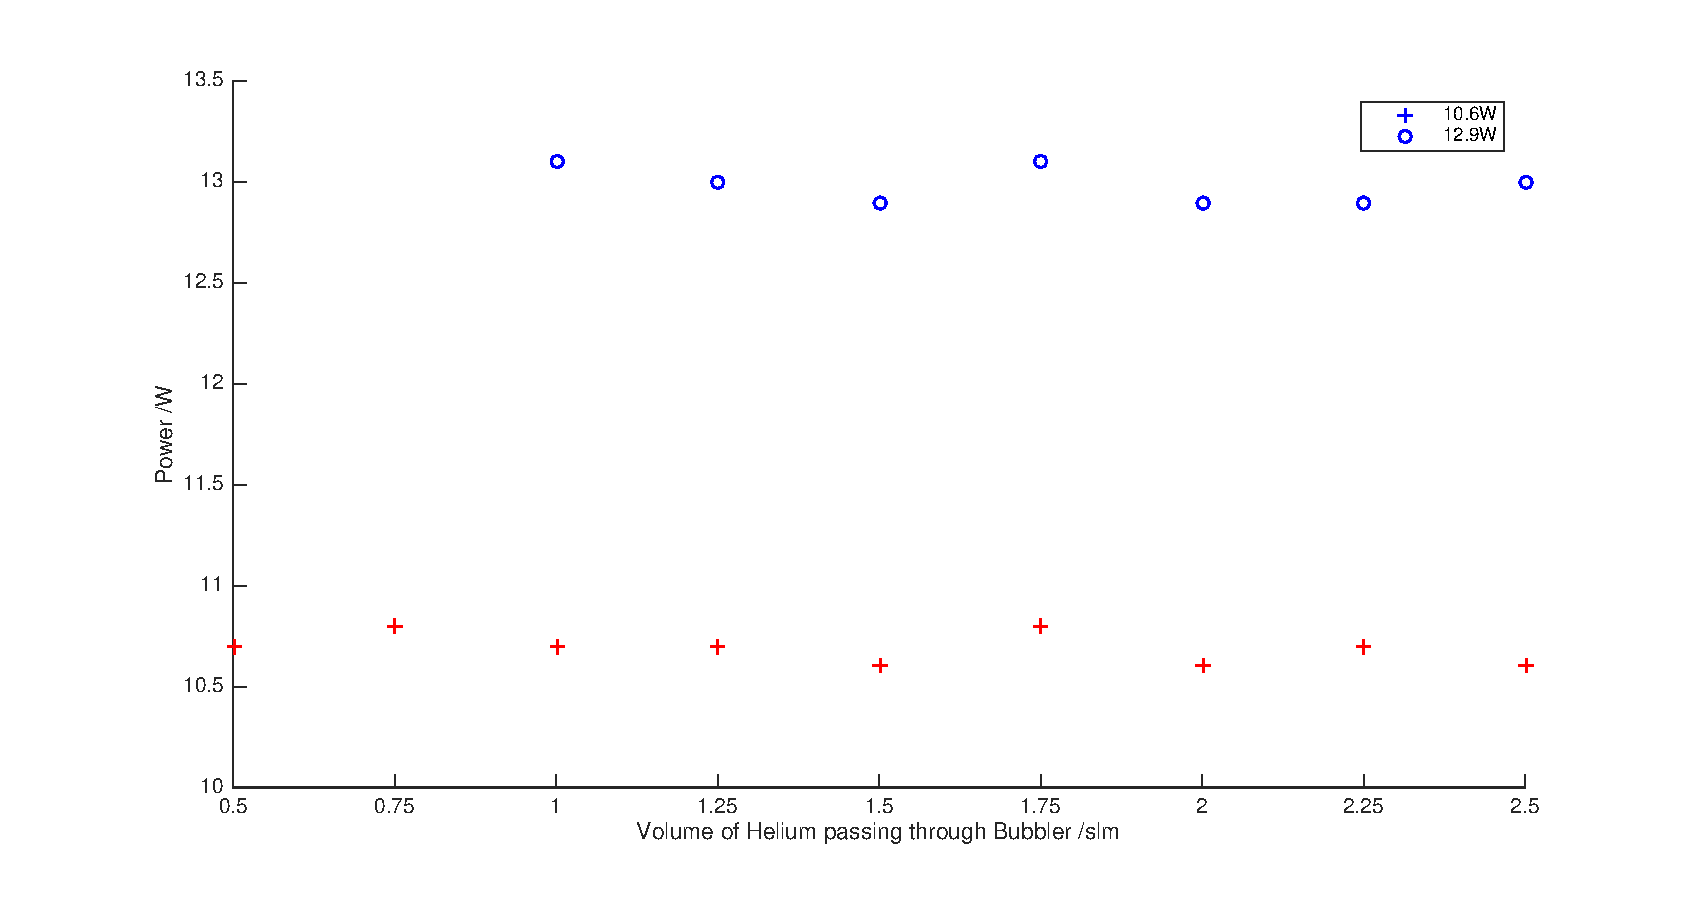
\includegraphics[width=\textwidth]{Figures/BubblerPower.eps}
    %\caption{The water content of the feed gas has no effect on the power supplied to the plasma. The water content of the feed gas was varied at high and low power. For each of the two powers, the output of the RF generator was kept constant and only the water content of the feed gas changed.}
    %\label{fig:BubblerPower}
%\end{figure}

\subsection{UV Absorption Spectroscopy}
To investigate the density of hydroxyl radicals present in the plasma, an ultraviolet (UV) light emitting diode (LED) with central wavelength of 309 nm (a wavelength specifically absorbed by free hydroxyl radicals \cite{Hatano2010}) was used for absorption spectroscopy.
The principle of this method is to measure the intensity of light before and after passing through the plasma, in order to see how much has been absorbed within the plasma by the species of interest.
In this case, the species of interest is the hydroxyl radical, therefore, the more hydroxyl radicals present in the plasma, the greater the absorbance of LED.
The UV beam passes through the plasma and a series of optics, then signal is detected by an imaging spectrograph with a (CCD) camera.

The transmittance of light beam and it's relationship to the absorbance is shown as follows:


\begin{equation} \label{eqn:Transmittance}
    T = \frac{I_T}{I_0} = e^{-A}
\end{equation}
Where $T$ is transmittance, $I_T$ and $I_0$ are the intensities of the transmitted and incident light, respectively and $A$ is the absorbance of light by the plasma.

In order to measure $I_T$ and $I_0$ for the plasma setup, it is necessary to measure four different parameters as follows:
\begin{itemize}
    \item $I_{PL}$ - The intensity of light reaching the CCD when both the LED and the plasma are on (figure \ref{subfig:Ipl})
    \item $I_{P}$ - The intensity of light reaching the CCD when the LED is off and the plasma is on (figure \ref{subfig:Ip})
    \item $I_L$ - The intensity of light reaching the CCD when the LED is on and the plasma is off (figure \ref{subfig:Il})
    \item $I_{BG}$ - The intensity of background light when both the LED and plasma are off (figure \ref{subfig:Ibg})
\end{itemize}

\begin{figure}
	\begin{subfigure}{0.2\textwidth}
  	  	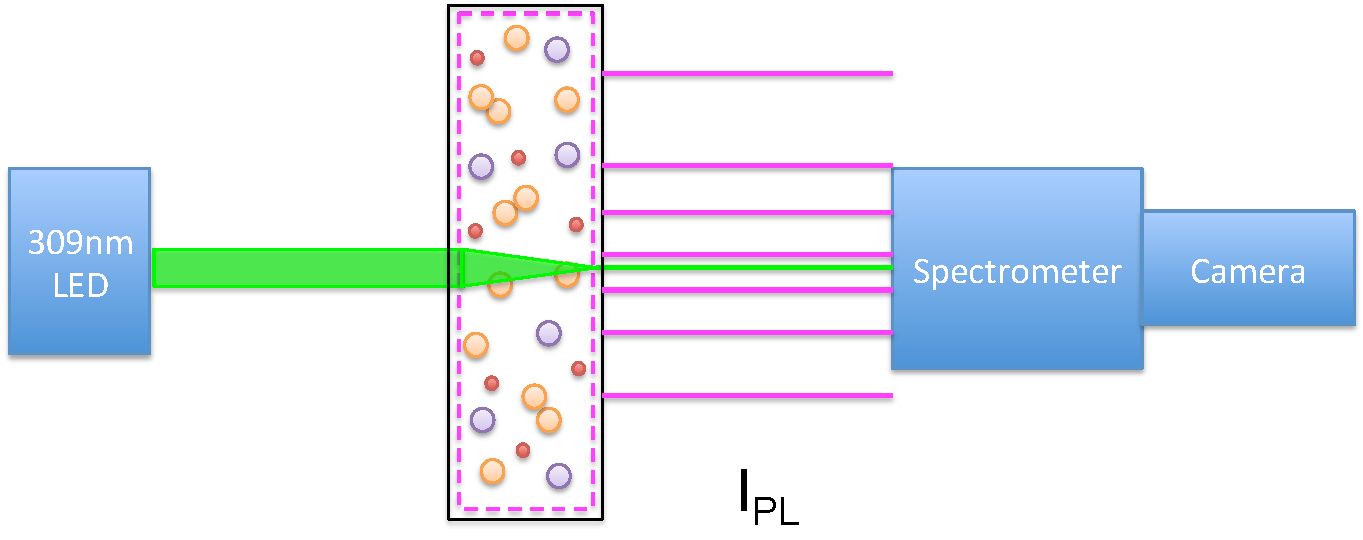
\includegraphics[width=\textwidth]{Figures/Ipl.pdf}
   	 	\caption{$I_{PL}$}
    		\label{subfig:Ipl}
	\end{subfigure}
	\hfill
	\begin{subfigure}{0.2\textwidth}
    		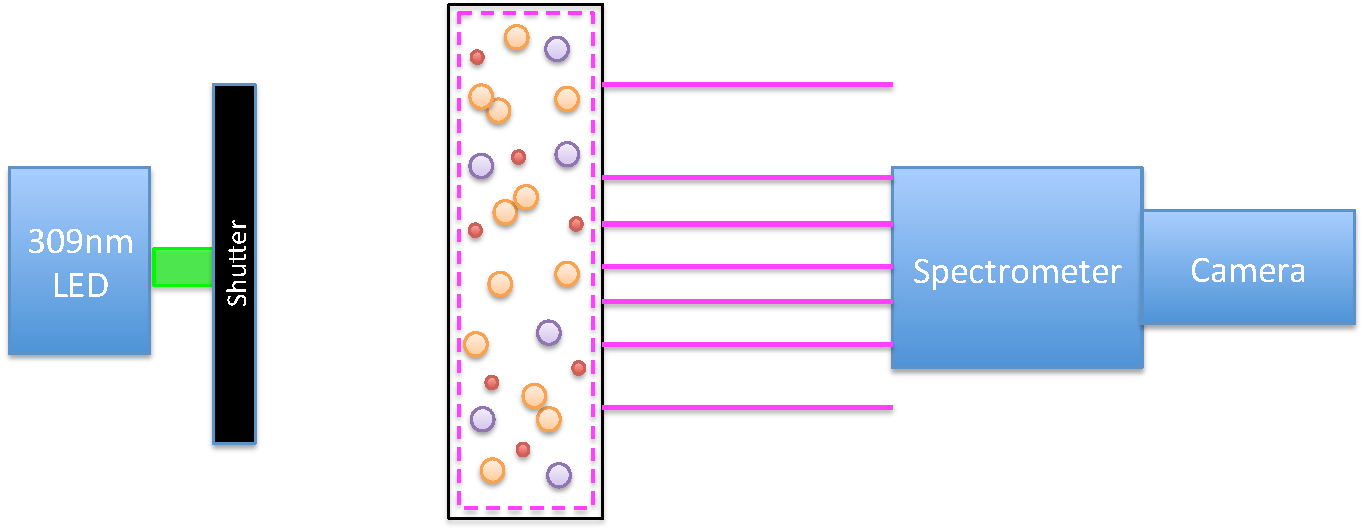
\includegraphics[width=\textwidth]{Figures/Ip.pdf}
    		\caption{$I_{P}$}
    		\label{subfig:Ip}
	\end{subfigure}
	\hfill
	\begin{subfigure}{0.2\textwidth}
		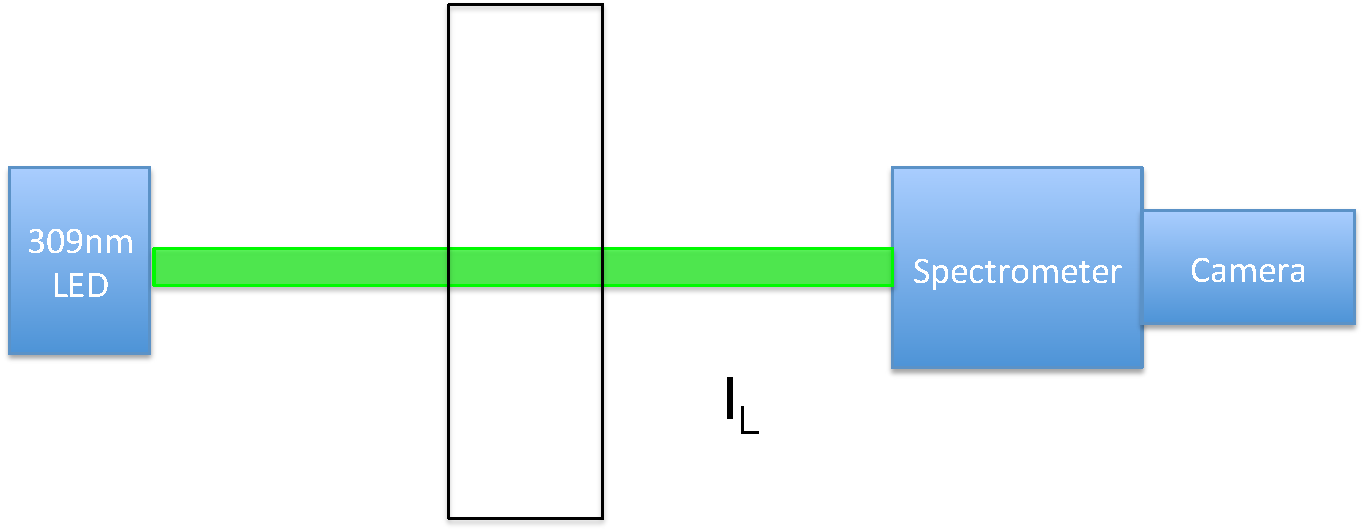
\includegraphics[width=\textwidth]{Figures/Il.pdf}
    		\caption{$I_{L}$}
		\label{subfig:Il}
	\end{subfigure}
	\hfill
    	\begin{subfigure}{0.2\textwidth}
    		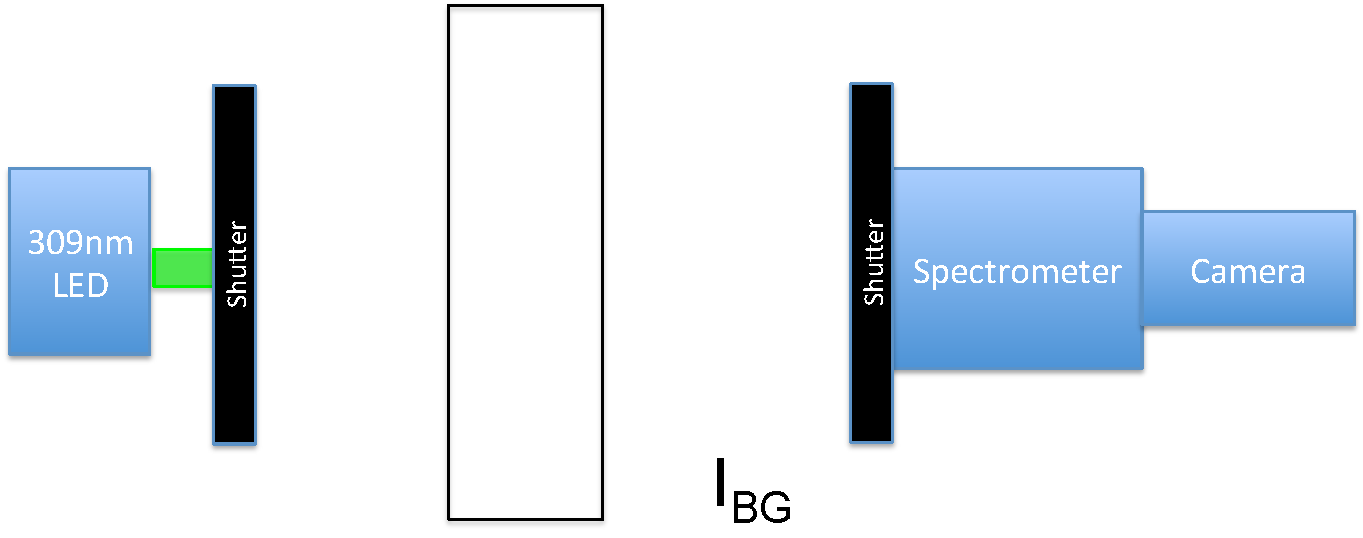
\includegraphics[width=\textwidth]{Figures/Ibg.pdf}
    		\caption{$I_{BG}$}
    		\label{subfig:Ibg}
	\end{subfigure}
	\caption{Rectangle represents plasma channel. Splodges are important bits of plasma. Green line is LED.}
\end{figure}

Using these measurements, the equation defining the relationship between transmittance and absorbance becomes:

\begin{equation} \label{eqn:4ParamTransmittance}
    T = \frac{I_T}{I_0} = \frac{I_{PL} - I_P}{I_L - I_{BG}} = e^{-A}
\end{equation}

All four parameters are measured in series, under the control of a function generator.
This function generator controls a shutter to block the LED and the RF generator to turn the plasma on and off. It also controls external triggering of the camera and a shutter at the entrance to the spectrometer to block all light to the CCD while the system changes from one parameter to the next. 

Data is then acquired as a series of 80 measurements resulting in 20 repeats for each of the four parameters.
Matlab is then used to average all 20 repeats for each parameter then calculate absorbance at each wavelength of the LED as follows:

\begin{equation}\label{eqn:Absorbance}
    A = -ln(\frac{I_{PL} - I_P}{I_L - I_{BG}})
\end{equation}

\subsection{Spectral fitting and radical density determination}

Once the absorbances for each wavelength have been calculated, a simulated spectrum can then be fitted to the data to provide a spectrum of absorbance for hydroxyl radicals (see figure \ref{fig:SpectrumFitting}). 
The spectrum shows absorption due to ground state hydroxyl radicals becoming rotationally and/or vibrationally excited.
In fitting this spectrum, the programme calculates the density of hydroxyl radicals present in the plasma.

\begin{figure}
    \centering
    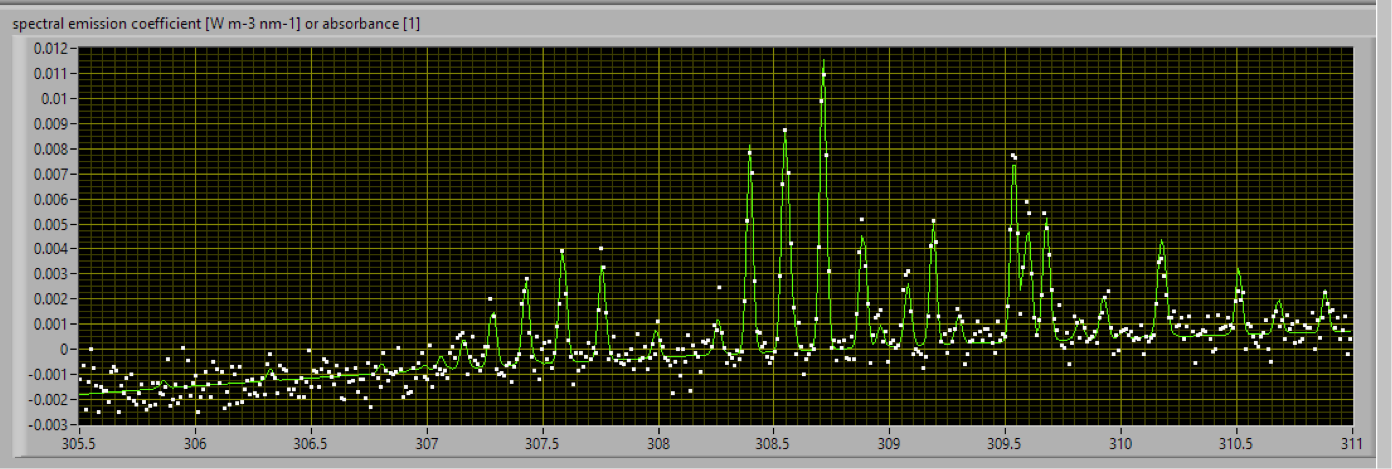
\includegraphics[width=\textwidth]{Figures/SpectrumFitting.png}
    \caption{An example of a simulated spectrum (green line) fitted to the measured absorbances (white dots). Wavelength is shown along the x axis and absorbances along the y axis.}
    \label{fig:SpectrumFitting}
\end{figure}

\subsection{Calculating the Water Content of Helium}
\label{subsec:CalculatingWaterContent}


To calculate the water content of helium passing through the bubbler, firstly, the flow of water must be determined. For this, the pressure of water vapour in the bubbler ($P_{water}$) is calculated using the following equation taken from reference \cite{Alduchov1996}:

\begin{equation}
	e_w = 6.1094 e^{\frac{17.625t}{243.04 + t}}
\end{equation}
Where $e_w$ is the water vapour pressure in hPa, above a plane surface of pure water, and $t$ is the temperature in degrees celsius.

The pressure of helium ($P_{He}$) is taken to be $P_{atmosphere} - P_{water}$. Since the ratio of flow to pressure for helium must be the same as for water, the flow of water can be calculated as follows:

\begin{equation}
    F_{water} = \frac{F_{He} * P_{water}}{P_{He}}
\end{equation}

Where $F_{water}$ and $F_{He}$ are the flows of water and helium in slm, respectively. The percentage of gas flow that is water, and the concentration of water in parts per million can then be determined.
The relationship between the flow of helium through the bubbler and the concentration of water in ppm is shown in figure \ref{fig:WaterContent}.

\begin{figure}
    \centering
    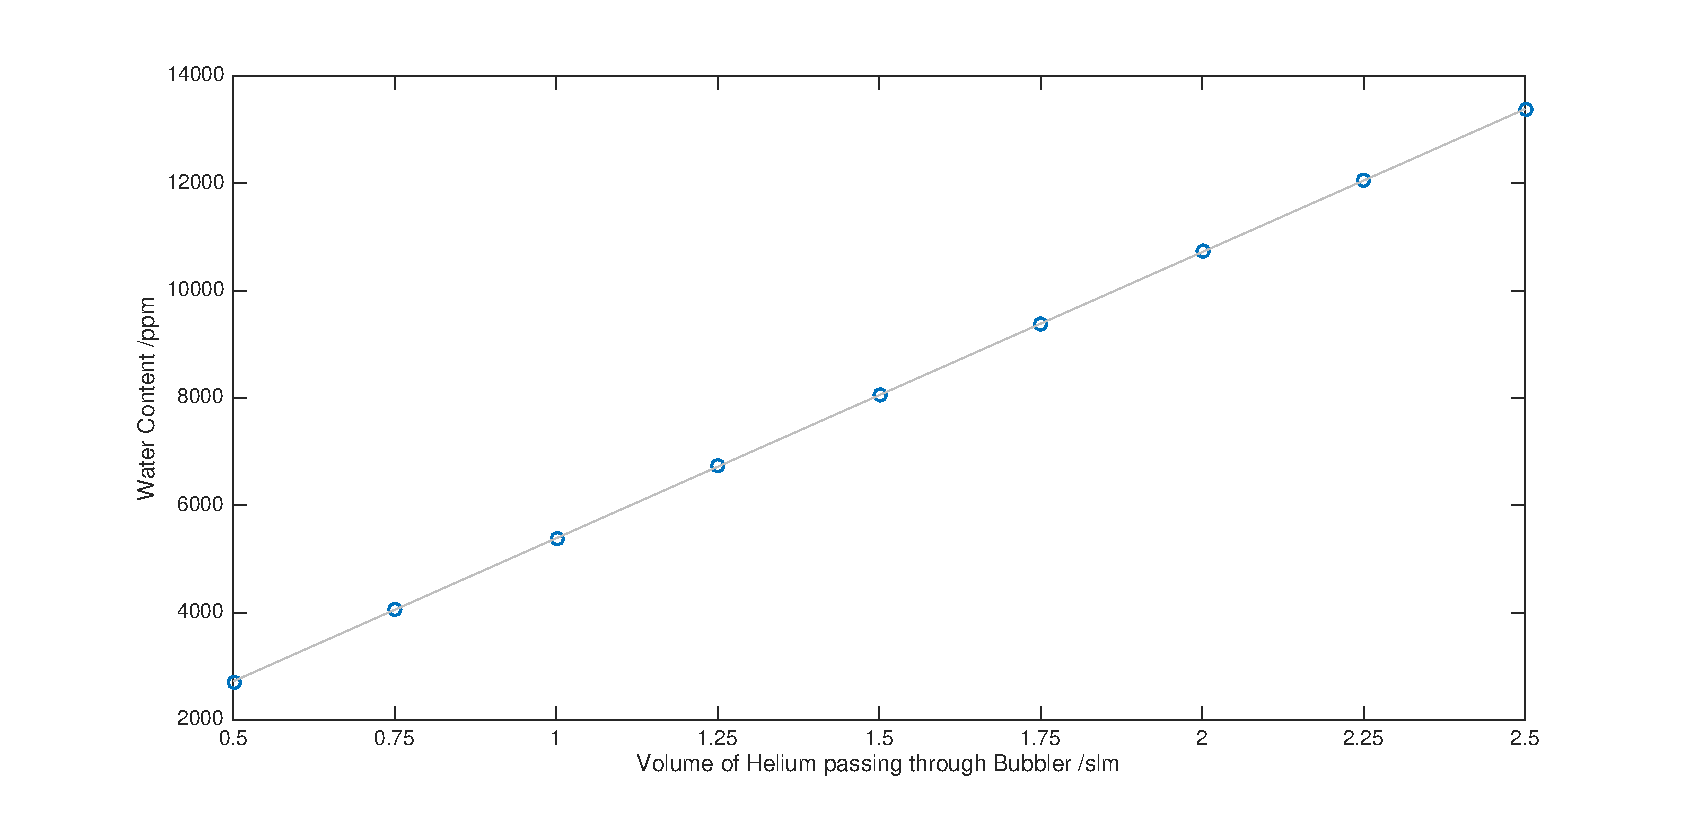
\includegraphics[width=\textwidth]{Figures/WaterContent.eps}
    \caption{The water content of the helium passing through the bubbler increases linearly with the volume of helium passing through the bubbler. Water content calculated using equation from \cite{Alduchov1996} and procedure described in the text.}
    \label{fig:WaterContent}
\end{figure}

%\subsection{Modelling of Hydroxyl Radical Production}

%\begin{itemize}
%\item Global model of plasma written by Sandra
%\item approximately 300 reactions taken into account and the probabilities that they will occur
%\item Coupled with gas flow rate, power, plasma volume and diffusion length
%\item Solves equations that take into account the probabilities of species being produced the different reactions (using the rate constants for each reaction), along with the rates of losses due to recombination.
%\item The data from the model can be compared to the experimental data
%\item Running the model then can give an indication of the dominant reactions for the production and loss of hydroxyl radicals
%\end{itemize}



\section{Results}

\subsection{Spatial Resolution of Hydroxyl Radicals} \label{subsec:SpatialRes}

\begin{figure}
    \centering
    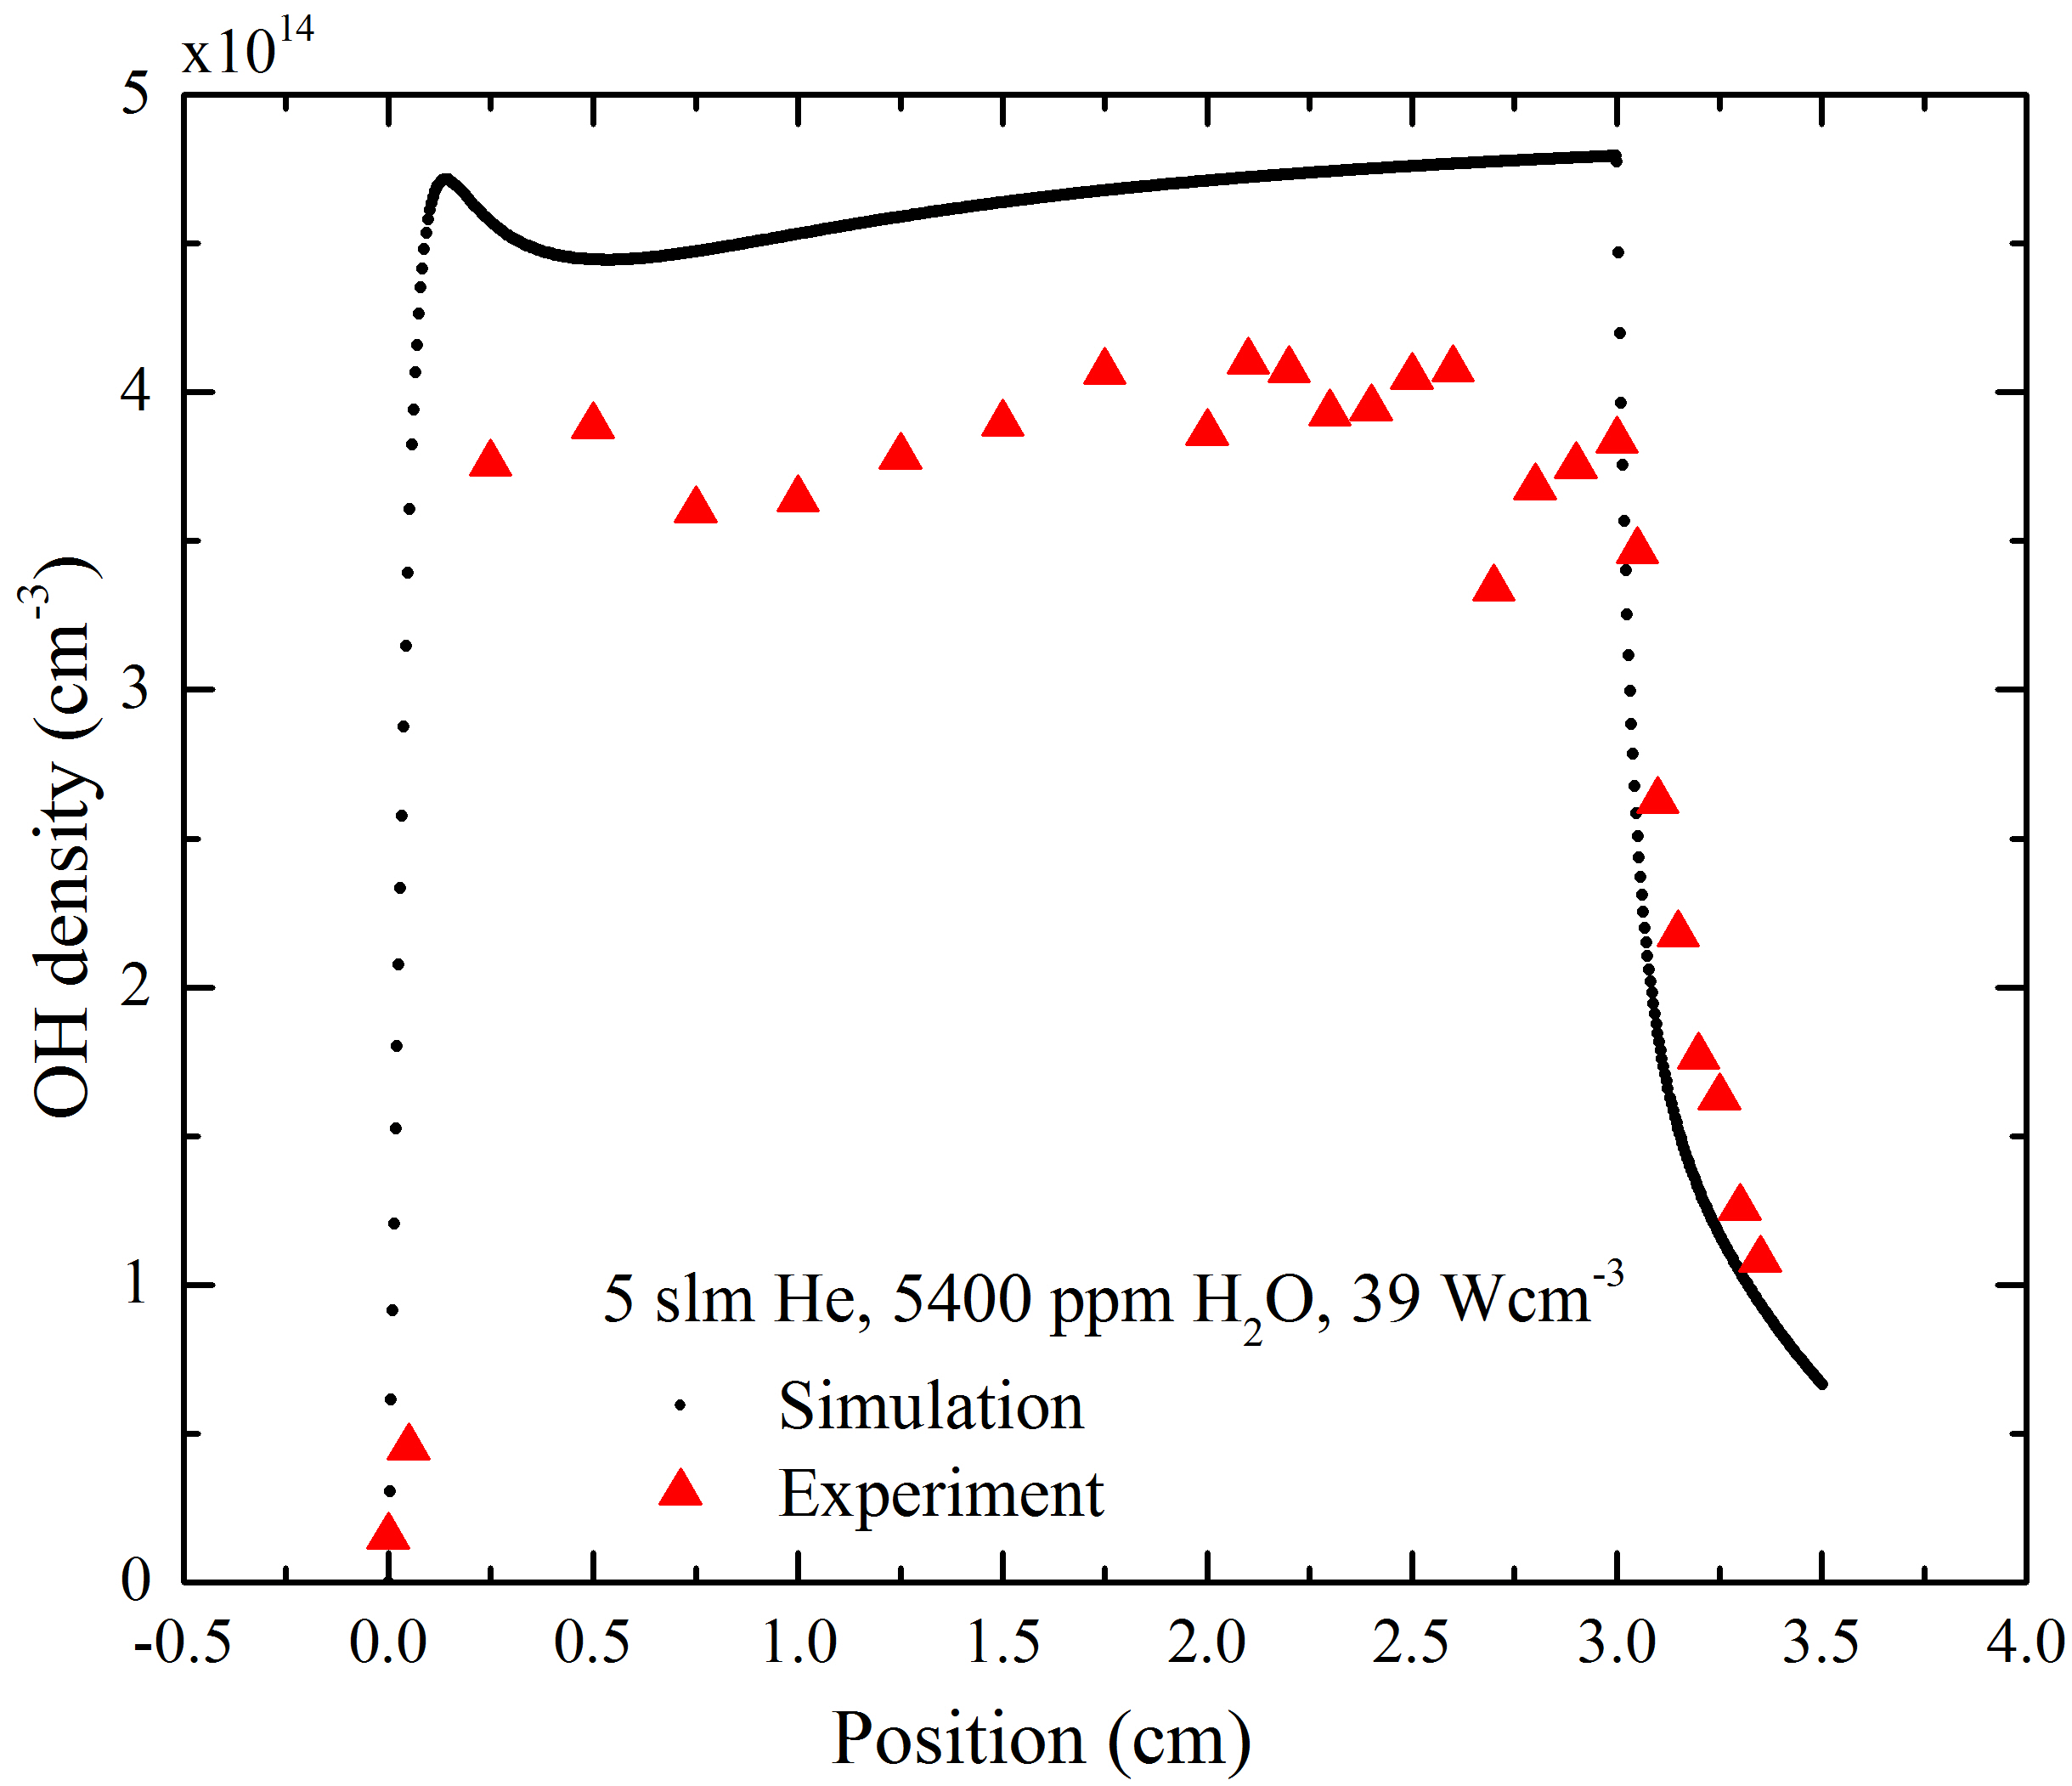
\includegraphics[width=\textwidth]{Figures/OHSpatialwithSim.jpg}
    \caption{Figure showing the effects of distance from gas inlet on the density of $\cdot$OH in plasma. Absorption spectroscopy was performed at 0.5 - 1mm intervals along the 30mm length of the electrodes (0-30mm), plus at 0.5mm intervals beyond the end of the plasma region (30.5-33.5mm). The position along the plasma channel in mm is shown on the x axis, and the corresponding $\cdot$OH density is shown in m\textsuperscript{-3} on the y axis. The plasma was operated at 10.9W with a feed gas flow rate of 5slm with 5400ppm water.}
    \label{fig:SpatialRes}
\end{figure}

\begin{figure}
	\centering
	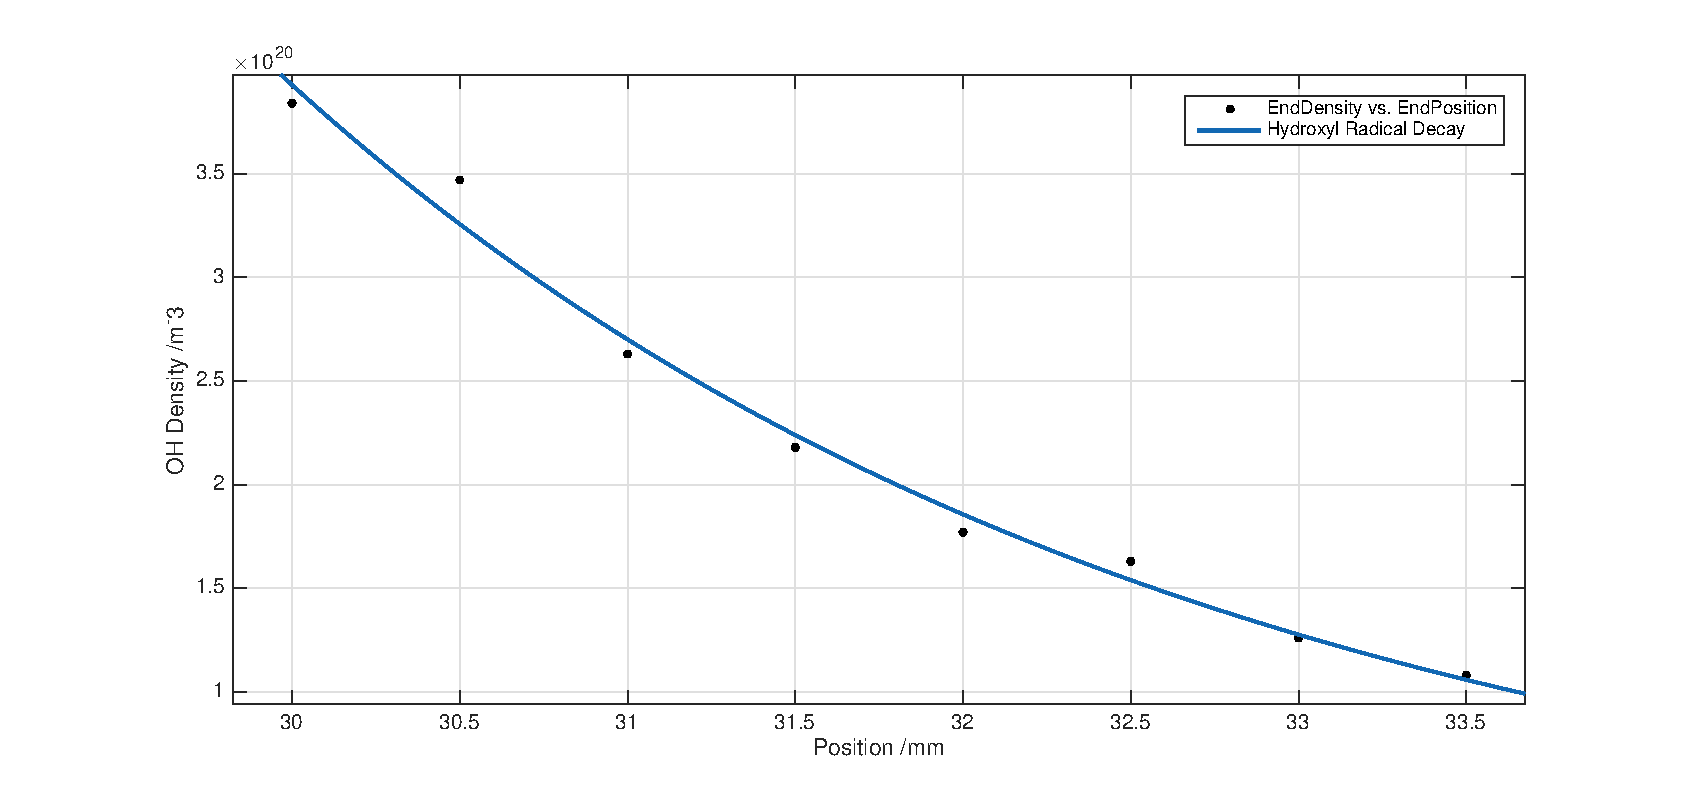
\includegraphics[width=\textwidth]{Figures/OHdecay.eps}
	\caption{Figure showing the rapid decay of $\cdot$OH beyond the ends of the plasma channel. The position in the plasma source is shown on the x axis in mm, and the corresponding $\cdot$OH density is shown in m\textsuperscript{-3} on the y axis. The 30mm point is the end of the electrodes and 33.5mm is the last point where the measurement could be taken before the LED was blocked by the casing of the plasma source. The plasma was operated at 10.9W with a feed gas flow rate of 5slm with 5400ppm water.}
	\label{fig:OH decay}
\end{figure}

The aim of this experiment was to show how the distance from the gas inlet, and therefore, the position along the 30mm electrode, affects the density of hydroxyl radicals. Figure \ref{fig:SpatialRes}.
Further to this, it was also possible to assess the densities of $\cdot$OH up to 3.5mm beyond the end of the electrodes, in order to assess the rate of decay of $\cdot$OH beyond the end of the plasma channel.
This is relevant when considering treatments using plasma jets where the biological sample is likely to be a short distance away from the end of the jet therefore, the species present at this point need to be assessed.
It also is able to provide information on the decay rate of hydroxyl radicals at the end of the electrodes.

To carry out the experiment, the highest power that can be supplied to the setup before causing arcing was used, 10.9W.
In addition to the measurements taken during the experiment, the data was also simulated using a model developed by Sandra Schr\"{o}ter (REFERENCE???).
This is a global model of the plasma which contains over 300 reactions for the production of $\cdot$OH along with their rate constants (probabilities that they will happen). It also takes into account the plasma conditions such as plasma volume, feed gas flow rate and power. 

The data acquired by both experiments (red triangles) and simulation (black dots) are shown in figure \ref{fig:SpatialRes}.
The graph shows that there is a sharp increase from 0-2.5mm, followed by a smaller increase and decrease to give a little hump seen in both the experimental and simulated data. Following this there is an increase in density over the rest of the channel.
Whilst the simulation and experimental data seem to fit nicely, it would be interesting to do further repeats of the experiment in order to check the match between simulation and experiment, and to get an idea of the error that can be expected in the experiment.
Overall there is the trend of a sharp increase at the start of the plasma channel, followed by a small increase and decrease, the a general increase in density to the end of the channel. 
However, the change in density is very small (less than 1 x 10\textsuperscript{20} m\textsuperscript{-3}), therefore it seems that the position along the plasma channel does not have a massive effect on the $\cdot$OH density.
Using data from the model, it appears that the dominant reaction for the formation of $\cdot$OH electron impact causing dissociation of H2O ($e^- + H_2O \rightarrow H + OH + e^-$), followed by $H + HO_2 \rightarrow OH + OH$.

To interrogate the decrease in $\cdot$OH density beyond the end of the electrodes, measurements were taken every 0.5mm from the end of the channel to the edge of the window.
A curve was then fitted to the data points to see the decay of hydroxyl radicals with distance from the end of the electrodes.
As shown, there is a rapid, significant decrease in $\cdot$OH density beyond the end of the electrodes.

By plotting the decay on a log scale, as shown in figure???????, it gives an idea as to how many decay processes are occurring. For example, the linear relationship seen over the full decay would suggest that there is one dominant decay process. 
The information provided by the model suggests that the dominant reaction causing loss of OH is $OH + H_2O_2 \rightarrow  HO_2 + H_2O$. However, it also suggests that there are other processes that are less important but still contributing, in particular $OH +HO_2 \rightarrow O_2 +H_2O$ and  $OH + OH \rightarrow H_2O_2$.
This would raise the question as to whether the model and experimental data actually match. The model would suggest there is more than one decay process, whereas the experimental data doesn't.
This could be explained by an error in alignment during the experimental process, whereby what is seemingly the end of the plasma channel, in fact, isn't. 
By elimating the first point from the analysis, it appears that the decay curve changes and looks less linear.
In the future, it would be of use to be able to make sure the plasma source is definitely fully aligned somehow so that the limits of the electrodes are well known.
Another difference between the model and the experimental setup for this decay region, is the fact that in the model, beyond the 30mm, there is no power at all. However, in the experimental setup, the casing of the source is acting as the grounded electrode and therefore continues further than the driven electrode. This could result in coupling between the driving and grounded electrode beyond the 30mm channel and influence $\cdot$OH.


Lifetime??


\subsubsection{The percentage dissociation is very small}

The degree of dissociation of water to hydroxyl radicals was then investigated by comparing the concentration of water entering the plasma (in this case 5400ppm), with the concentration of $\cdot$OH in the plasma.
The percentage dissociation was then calculated as follows:

\begin{equation} \label{eqn:PercentDiss}
	\frac{concentration \cdot OH}{concentration  H_2O} \times 100
\end{equation}

By calculating this for each point along the channel, it showed that the percentage dissociation of water to $\cdot$OH was very small (\textless 0.35\%), see figure \ref{fig:SpatialDissociation}.
However, while these numbers seemingly show that only a small amount of the water is dissociating, it may also be that $\cdot$OH are recombining with other things very rapidly and are therefore being lost.

\begin{figure}
	\centering
	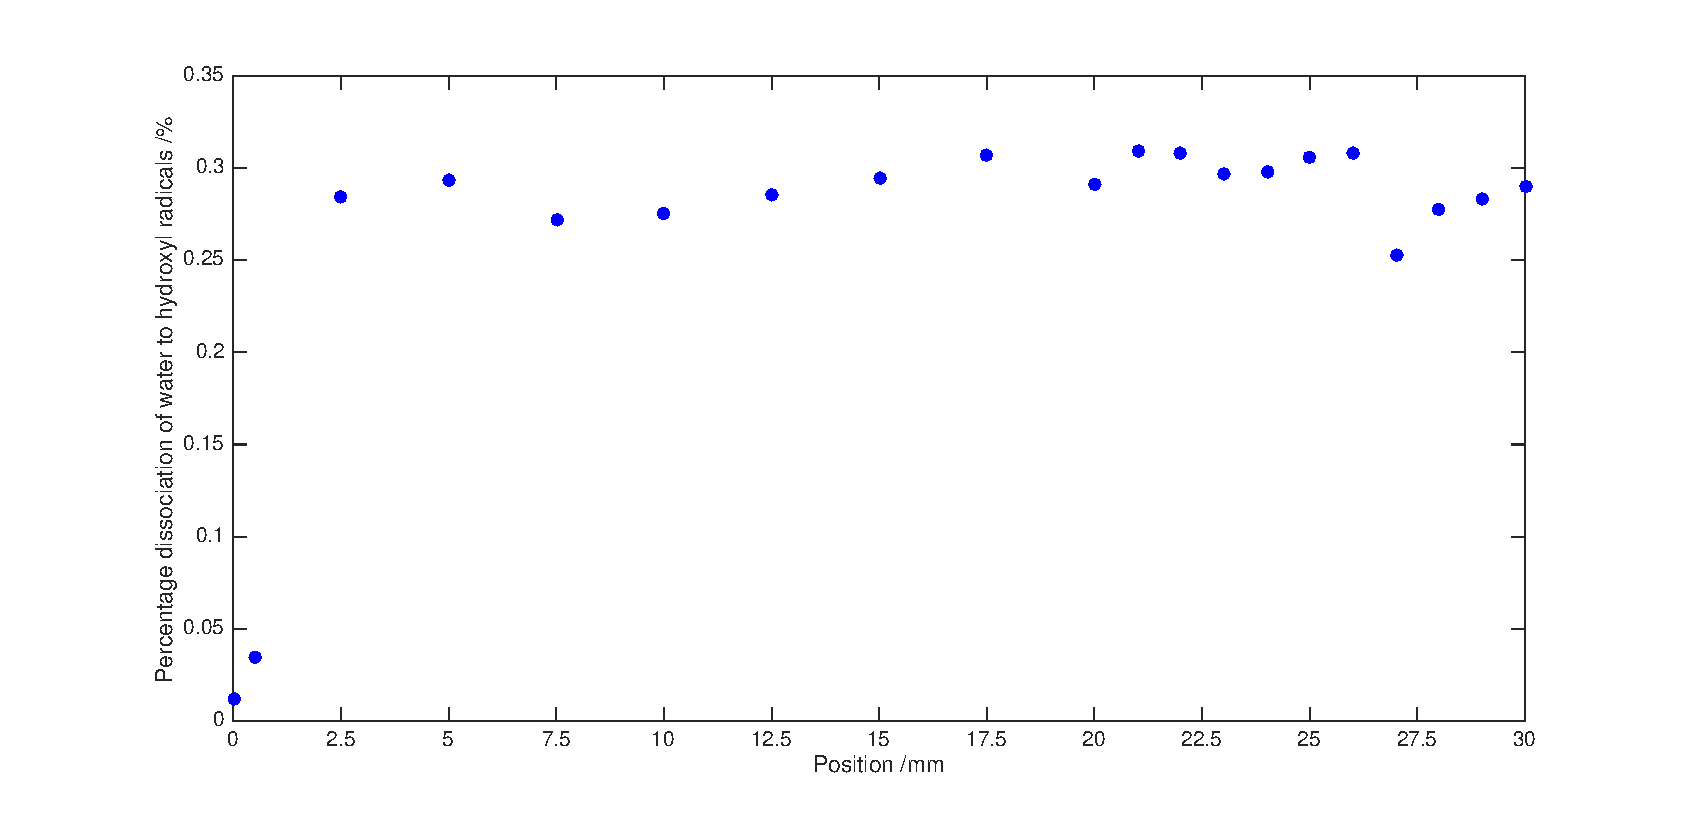
\includegraphics[width=\textwidth]{Figures/SpatialDissociation2.eps}
	\caption{The figure shows the percentage dissociation of water to hydroxyl radicals, calculated as ppm hydroxyl radicals divided by ppm water in, all multiplied by 100. Since the ppm of water stays the same at all positions, the graph shows the same trend as the equivalent density graph.}
	\label{fig:SpatialDissociation}
\end{figure}


\subsection{Increasing the power to the plasma increases hydroxyl radical density}

Following investigation of the spatial resolution of hydroxyl radicals, the effects of power variation were then investigated.
It was of interest to see how varying the power would affect the density of hydroxyl radicals and the percentage dissociation of water to hydroxyl.
The 20mm position was chosen to investigate as at this point, as the spatial resolution data shown in figure \ref{fig:SpatialRes} show that $\cdot$OH densities seem to level off slightly. 
The full range of powers for the plasma were tested from 6.5W (minimum power for sustaining the plasma) to 10.9 W (maximum power before arcing occurs) and results of this are shown in figure \ref{fig:PowerVariation}.

The results show that the density of $\cdot$OH increase non-linearly with increasing power being supplied to the plasma, with a density range of approximately 3.25 - 4.5 x 10\textsuperscript{20} m\textsuperscript{-3}.
The experiment was repeated four times, meaning that a mean and standard deviation could be calculated from the data and is shown in the figure. 
This also gives an indication of the expected error in the experiment which is approximately $\pm$ 0.5 x 10\textsuperscript{20} m\textsuperscript{-3}.

\begin{figure}
    \centering
    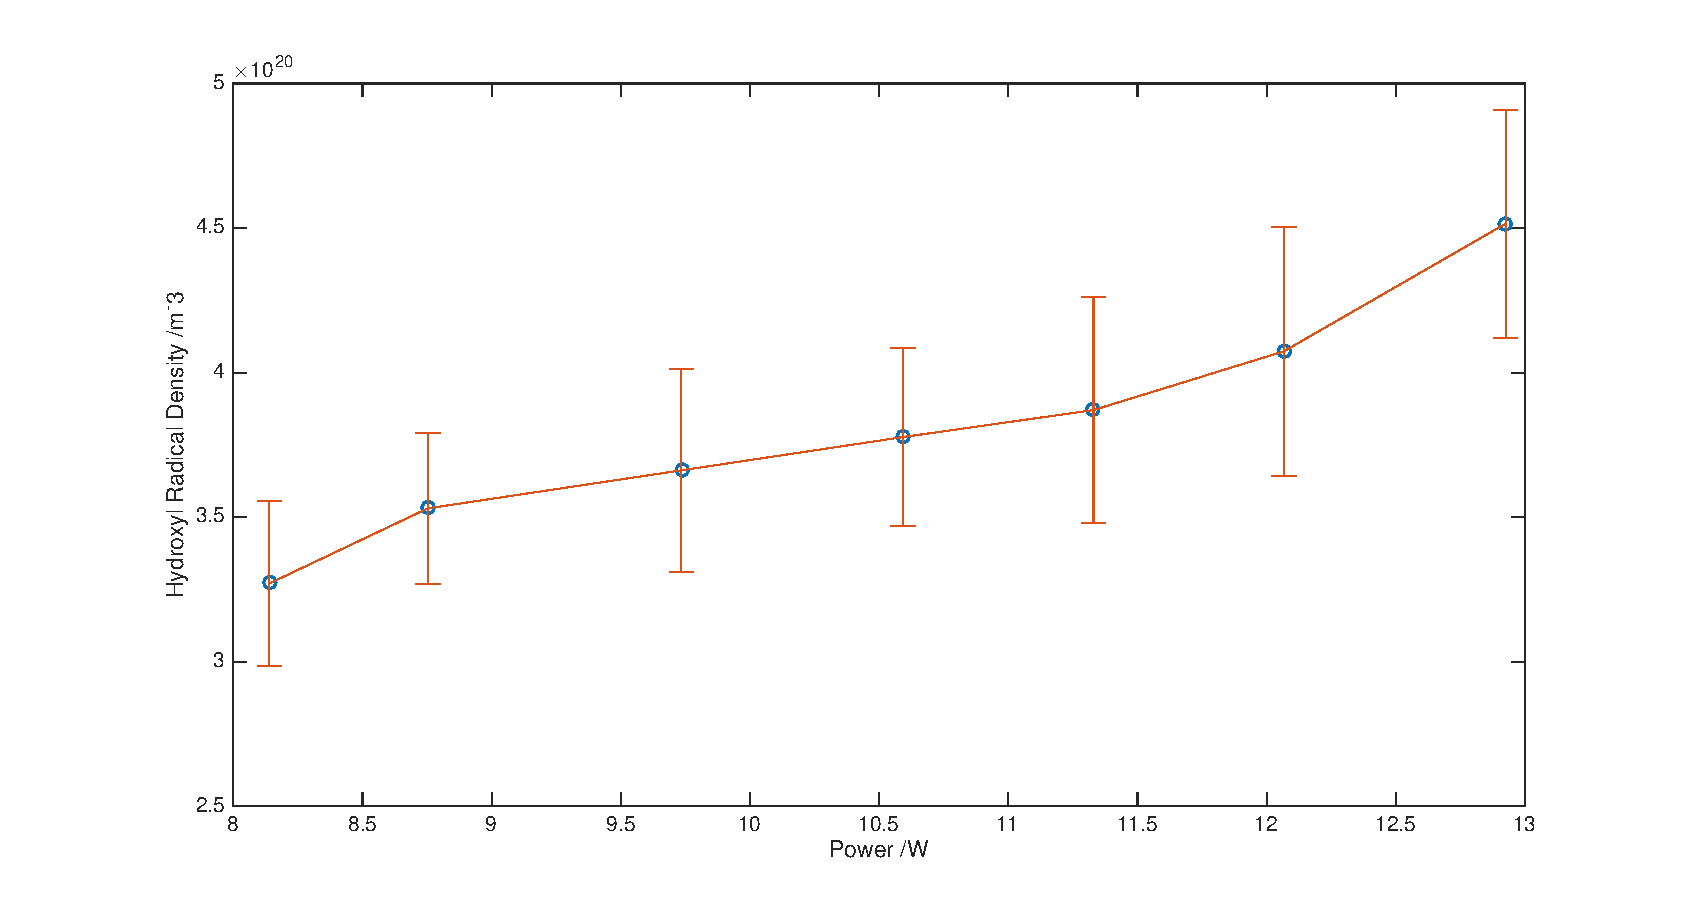
\includegraphics[width=\textwidth]{Figures/PowerVariation.eps}
    \caption{Power increases $\cdot$OH density in the plasma region in a non-linear manner. Absorption spectroscopy was performed at a point 20mm from the gas inlet while power being dissipated in the plasma was varied within the range of 6.5 - 10.9W, as shown on the x axis (CHANGE POWERS ON GRAPH). Total gas flow to the plasma was kept constant at 5slm helium with 5400ppm water. The experiment was repeated four times. The graph shows the average density (shown on the y axis in m\textsuperscript{-3}) for each power and the error bars represent one standard deviation.}
    \label{fig:PowerVariation}
\end{figure}

\subsubsection{Dissociation}

As in section \ref{subsec:SpatialRes}, the percentage dissociation of water to $\cdot$OH was calculated using equation \ref{eqn:PercentDiss}, and the percentage dissociation at the corresponding powers are shown in figure \ref{fig:PowerDissociation}.
Once again, the percentages seem extremely small at 0.24 - 0.34\% which, as mentioned previously, could be due to a genuine low level of dissociation, or it may be that the $\cdot$OH molecules are recombining too rapidly to be seen.
%Would it be possible to measure water content in the feed gas and the undissociated water in the plasma to see how much is actually left undissociated?
There is a trend of increasing dissociation with increasing power, however, unfortunately the power cannot be increased any further in this setup due to arcing occurring at powers higher than 10.9W.
Instead of this, it would be of interest to increase the frequency driving the electrodes and see what effect this has on the $\cdot$OH density.
Like increasing the power, increasing the frequency should increase the energy in the system which should, in turn increase the dissociation of water and increase the density of $\cdot$OH.

\begin{figure}
    \centering
    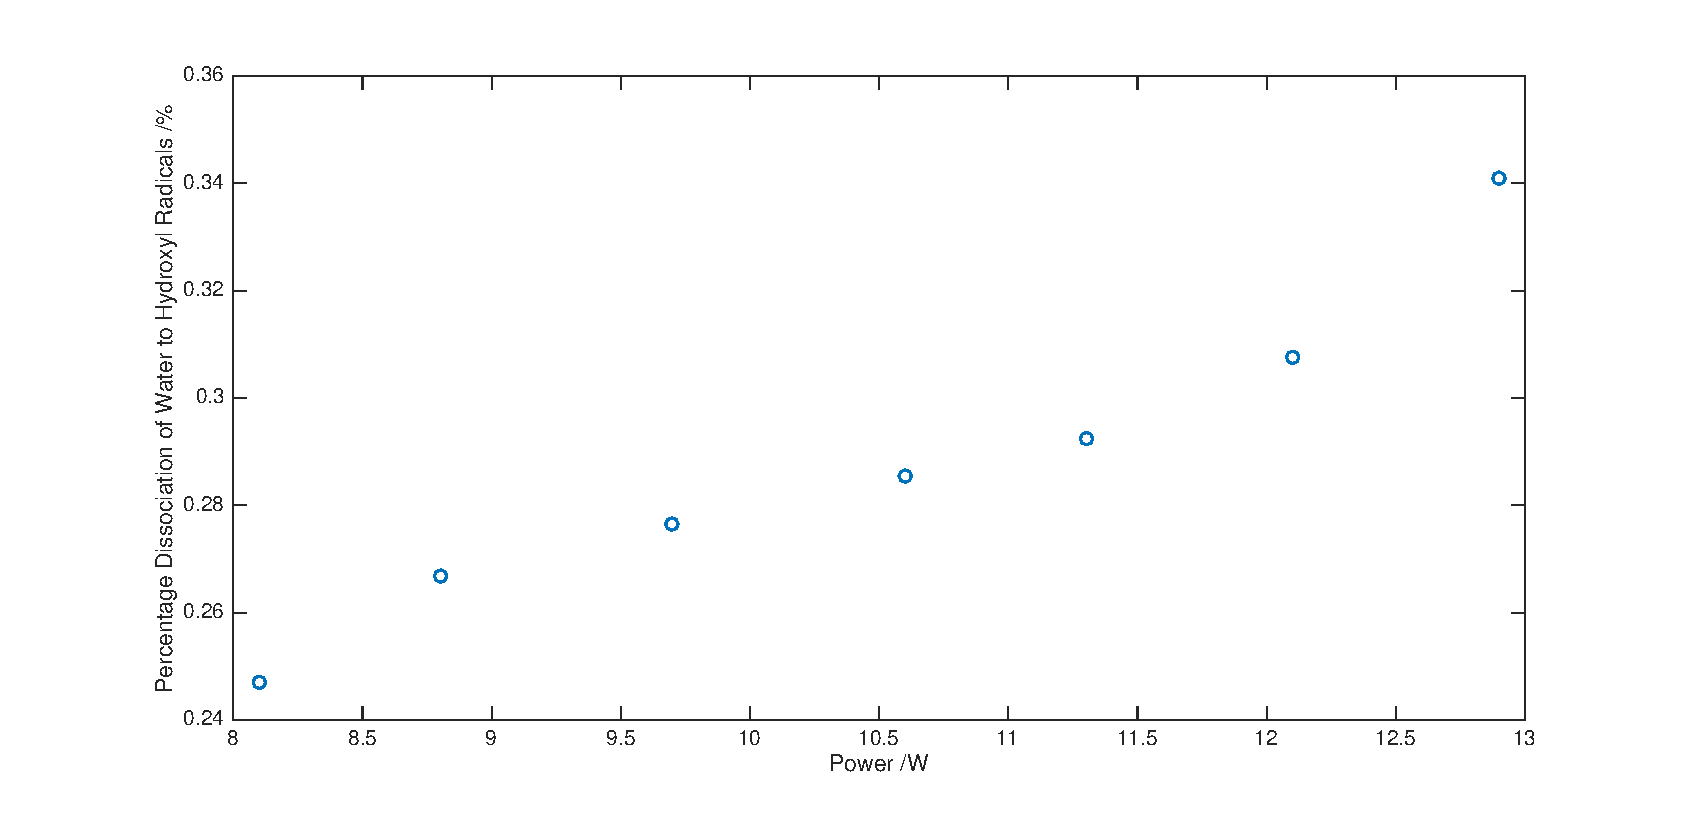
\includegraphics[width=\textwidth]{Figures/PowerDissociation.eps}
    \caption{The percentage dissociation of water to $\cdot$OH increases with increasing power. Absorption spectroscopy was performed at a point 20mm from the gas inlet. The plasma was operated with a total gas flow of 5slm helium plus 5400ppm water. The power range was 6.5 - 10.9W, as shown on the x axis and the corresponding percentage dissociation (calculated using equation \ref{eqn:PercentDiss} and the average $\cdot$OH densities shown in figure \ref{fig:PowerVariation}) is shown on the y axis. (CHANGE POWERS ON GRAPH)}
    \label{fig:PowerDissociation}
\end{figure}

\subsection{Increasing the water content of the plasma gas feed increases hydroxyl radical density}

To investigate whether increasing the water being fed to the plasma increases the hydroxyl radical density, the ratio of dry and humid helium entering the plasma channel was altered by changing the proportion of the total 5 slm helium that passed through the bubbler. The range of water concentrations entering the plasma was approximately 2700 - 13400 ppm. The results are shown in figure \ref{fig:BubblerVariation}.

The powers had to be carefully chosen due to the effects of adding in additional molecules into the plasma which can act as energy sinks when they absorb energy to change rotational and vibrational states. 
Therefore, higher water contents require higher powers to ignite as the system becomes less efficient when more molecules are added.
Two different powers were used to investigate the effects of altering the water content. Firstly, 8.7W was used as this was sufficient to sustain the plasma at high water contents, without causing arcing at low contents. Secondly, the power was increased to 10.9W to see how the density increased at the higher power. 

The results shown in figure \ref{fig:BubblerVariation} suggest that $\cdot$OH density increases when the water content of the feed gas increases. This is not unreasonable as in section \ref{subsec:SpatialRes}, it was discussed that the main reaction that resulted in $\cdot$OH production is electron impact with water, therefore the more water present, the greater the $\cdot$OH production.
The graph shows a similar, non-linear trend to both the high and low power data sets, whereby the density increases with increasing water content.
%However, particularly at the lower power, it appears that the densities increase fairly quickly between approximately 2500 - 7000 ppm of water, before starting to level off.
%This would suggest that maybe lower water contents would be interesting to investigate?

\begin{figure}
    \centering
    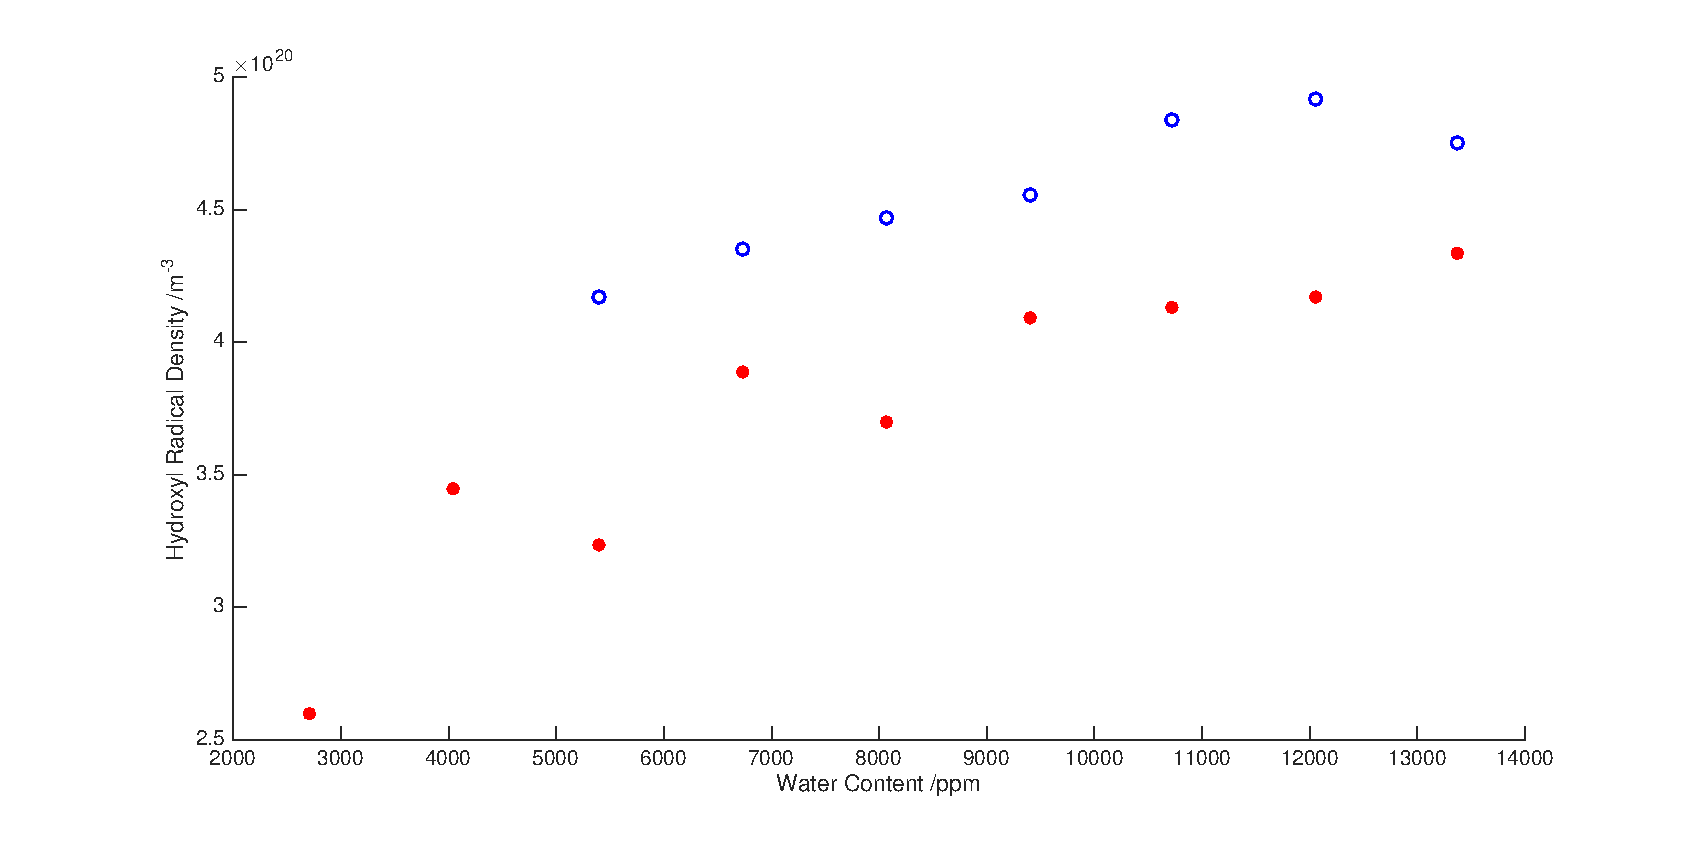
\includegraphics[width=\textwidth]{Figures/BubblerVariation}
    \caption{Increasing the water content of the plasma feed gas increases $\cdot$OH density in the plasma. Absorption spectroscopy of the plasma was performed at 20mm from the gas inlet to determine $\cdot$OH density (shown on the y axis). A total gas flow of 5 slm was maintained throughout, with differing water contents, ranging from 2700 - 13400 ppm (shown on the x axis). The powers used were 8.7W (red, filled dots) and 10.9W (blue, open dots)}
    \label{fig:BubblerVariation}
\end{figure}


\subsubsection{Dissociation}

Once again, the percentage dissociation of water to $\cdot$OH was calculated using \ref{eqn:PercentDiss} and the results are shown in \ref{fig:BubblerDissociation}.
Interestingly, with increasing water content, the percentage dissociation decreases in the plasma, despite the density of $\cdot$OH increasing.
This is seen for both the low and high power, though the percentages are higher for the higher power, as expected.

The decrease in percentage dissociation could be explained by the fact that increasing the water content of the plasma, increases the number of molecules present which, in turn, decreases the efficiency of the system.
The increase in water content means that more of the energy in the plasma system can be absorbed by the molecules in rotationally and vibrationally excited states.
This results in less energy available for electron processes such as dissociation, electronic excitation and ionisation (see section \ref{section:LowTempPlasmas}).




\begin{figure}
    \centering
    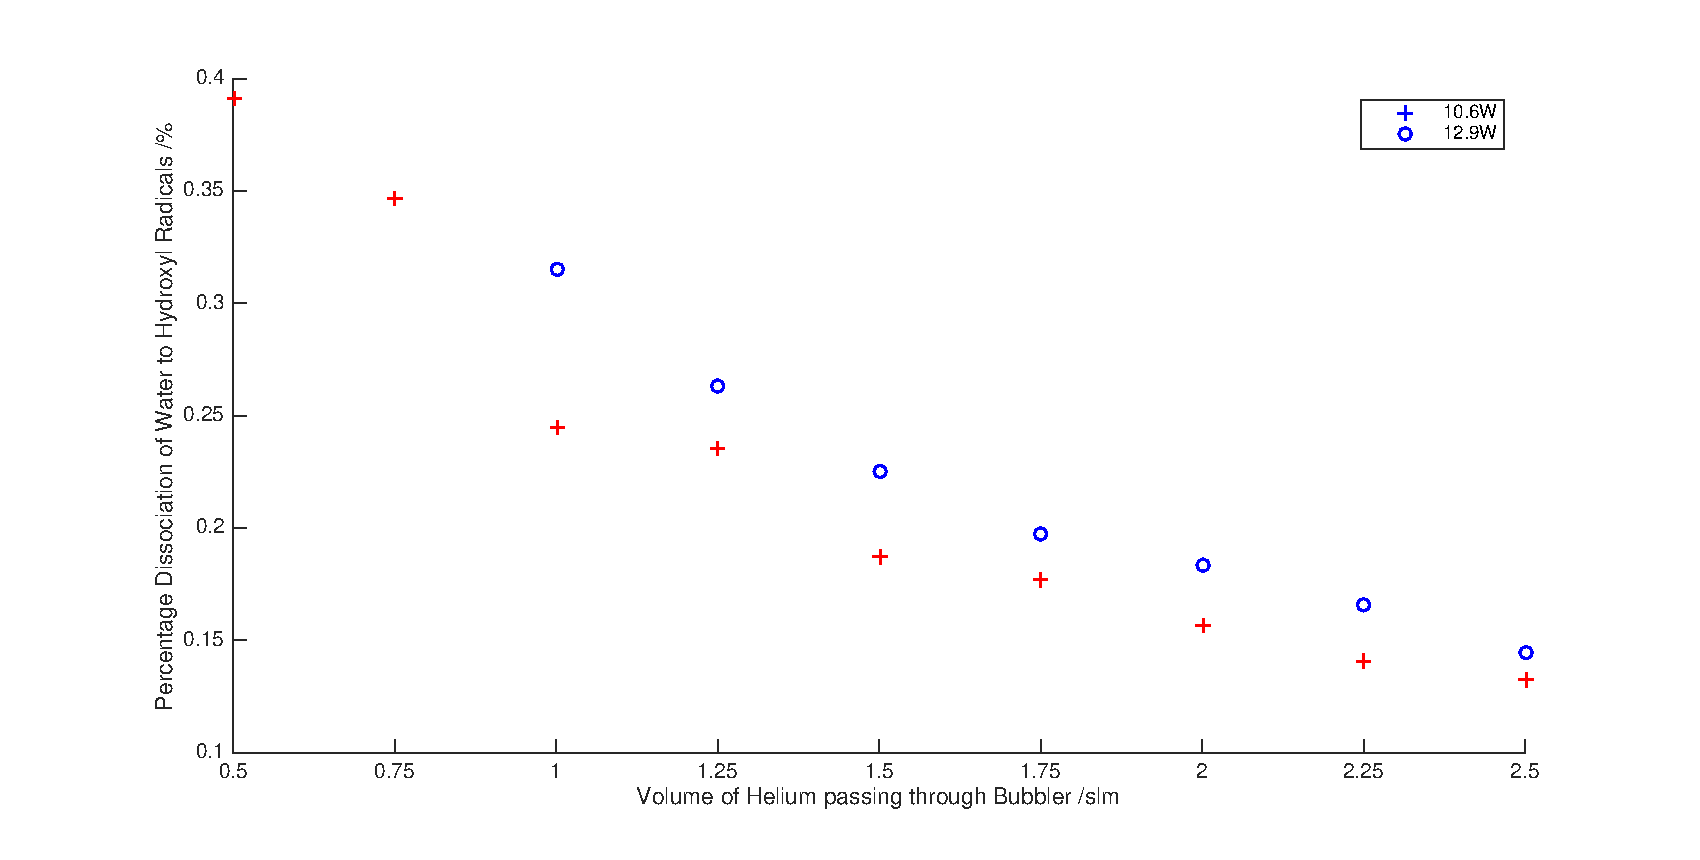
\includegraphics[width=\textwidth]{Figures/BubblerDissociation.eps}
    \caption{The percentage dissociation of water to hydroxyl radicals decreases as the water content increases. Absorption spectroscopy was carried out at a point 20mm from the gas inlet. The plasma was operated with a total of 5slm helium with water contents of 2700 - 13400 ppm. The experiment was repeated at two different powers of 8.7W (red crosses) and 10.9W (blue circles). (CHANGE GRAPH TO PPM WATER)}
    \label{fig:BubblerDissociation}
\end{figure}

\begin{itemize}
    \item Percentage dissociation decreases with increasing water content, despite the density of hydroxyl radicals increasing (see figure \ref{fig:BubblerVariation}). However, the water content increases more than the density, therefore the ratio of hydroxyl radical to water still decreases.
    \item The dissociation is higher for the higher power than the lower power, as would be expected. 
    \item Dissociation may also decrease due to the increase in energy absorption by molecules. The increase in water content means that more of the energy in the plasma system can be absorbed by the molecules in rotationally and vibrationally excited states. Could add oxygen into the feed gas. In theory, oxygen addition could increase hydroxyl radical density as, when water dissociates, there is a spare hydrogen which could combine with oxygen to form hydroxyl. However, this may have the opposite effect because, once again, a molecule is being added which could contribute further to the absorption of energy from the system. The oxygen would also require energy to be atomised before it could form $\cdot$OH with the spare hydrogen from water.
\end{itemize}




\section{Discussion}

Discuss lots of important things here!!!!! Woo!

\begin{itemize}
\item Increasing frequency to increase dissociation (can't increase power)
\item Change/adapt source to allow better interrogation of effluent
\item Alignment issues - improve the setup reduce error from twisting/moving of source when moving the stage vertically. Make sure everything is properly level to stop movement in x direction when moving in y direction.
\item Try to accurately identify the ends of the electrodes rather than guess
\item Test model more - change water content and see how it matches

\item Understand dose-response of plasma treatments. How long would it need to be treated and how many times? Is there a threshold for damaging host cells too much? Is it like chemotherapy needing recovery time between treatments? 
\item Selectivity. Is there a way of making these treatments selective only against bacteria, not host cells
\item Could antibiotics be aerosolised into the plasmas? Immunotherapy?!
%\item Big picture - develop a plasma jet that can kill off all bacteria in a big wound in wildlife so that they can be treated once to avoid the need to capture etc

\end{itemize}

\bibliographystyle{unsrt}
\bibliography{MyPapers}

\end{document}  